% Full instructions available at:
% https://github.com/elauksap/focus-beamertheme

\documentclass[9pt]{beamer}
\usetheme{focus}

%%%%%%%%%%%%%%%%%%%%%%%%%%%%%%%%%%%%%%%%%%%%%%%%%%%%%%%%%%%%%%%%%%%%%
% Typography, change document font
\usepackage[tt=false, type1=true]{libertine}
\usepackage[varqu]{zi4}
\usepackage[libertine]{newtxmath}
\usepackage[T1]{fontenc}

\usepackage[protrusion=true,expansion=true]{microtype}

% Disable paragraph indentation, and increase gap
\usepackage{parskip}

%Matrix
\usepackage{tabstackengine}
\setstackEOL{;}% row separator
\setstackTAB{,}% column separator
\setstacktabbedgap{1ex}% inter-column gap 
\setstackgap{L}{1.0\normalbaselineskip}% inter-row baselineskip
\let\mat\bracketMatrixstack

\newcommand{\pth}{Figure/}
\newcommand{\ve}[1]{\mathbf{#1}}

% Copyright (C) 2018-2019 Pasquale Claudio Africa and the LaTeX community.
% A full list of contributors can be found at
%
%     https://github.com/elauksap/focus-beamertheme
% 
% This file is part of beamerthemefocus.
% 
% beamerthemefocus is free software: you can redistribute it and/or modify
% it under the terms of the GNU General Public License as published by
% the Free Software Foundation, either version 3 of the License, or
% (at your option) any later version.
% 
% beamerthemefocus is distributed in the hope that it will be useful,
% but WITHOUT ANY WARRANTY; without even the implied warranty of
% MERCHANTABILITY or FITNESS FOR A PARTICULAR PURPOSE. See the
% GNU General Public License for more details.
% 
% You should have received a copy of the GNU General Public License
% along with beamerthemefocus. If not, see <http://www.gnu.org/licenses/>.

\mode<presentation>


% DEFINE COLORS. ---------------------------------------------------------------
\definecolor{main}{RGB}{134, 161, 174}
\definecolor{main2}{RGB}{104, 131, 144}
\definecolor{textc}{RGB}{20, 20, 20}
\definecolor{background}{RGB}{255, 255, 255}

\definecolor{alert}{RGB}{180, 0, 0}
\definecolor{example}{RGB}{0, 110, 0}


% SET COLORS. ------------------------------------------------------------------
\setbeamercolor{normal text}{fg=textc, bg=background}
\setbeamercolor{alerted text}{fg=textc}
\setbeamercolor{example text}{fg=textc}

\setbeamercolor{titlelike}{fg=background, bg=main}
\setbeamercolor{frametitle}{parent={titlelike}}

\setbeamercolor{footline}{fg=background, bg=main2}

\setbeamercolor{block title}{bg=main!80!background, fg=background}
\setbeamercolor{block body}{bg=main!10!background, fg=textc}

\setbeamercolor{block title alerted}{bg=alert, fg=background}
\setbeamercolor{block body alerted}{bg=alert!10!background, fg=textc}

\setbeamercolor{block title example}{bg=example, fg=background}
\setbeamercolor{block body example}{bg=example!10!background, fg=textc}

\setbeamercolor{itemize item}{fg=textc}
\setbeamercolor{itemize subitem}{fg=textc}

\setbeamercolor{enumerate item}{fg=textc!70!black}
\setbeamercolor{enumerate subitem}{fg=textc!70!black}

\setbeamercolor{description item}{fg=textc!70!black}
\setbeamercolor{description subitem}{fg=textc!70!black}

\setbeamercolor{caption name}{fg=textc}

\setbeamercolor{section in toc}{fg=textc}
\setbeamercolor{subsection in toc}{fg=textc}
\setbeamercolor{section number projected}{bg=textc}
\setbeamercolor{subsection number projected}{bg=textc}

\setbeamercolor{bibliography item}{fg=main}
\setbeamercolor{bibliography entry author}{fg=main!70!black}
\setbeamercolor{bibliography entry title}{fg=main}
\setbeamercolor{bibliography entry location}{fg=main}
\setbeamercolor{bibliography entry note}{fg=main}

\mode<all>


\begin{document}
	\tableofcontents

\section{Nonlinear Bending of straight beams : \today}
	\begin{frame}{Introduction}
		\begin{itemize}
			\item Assuming he geomery does no change significanty, allows he principle of virtual work o be written over the underformed body. So stress is force per unit undeforemed are, strain measure of change in length w.r.t original length and shear as change in length from $\pi/2$. No distincion between Piola kirchoff and cauchy stress
			\item Nonlinearity comes solely from inplane forces proportional to he square of the rotation of a transverse normal line in the beam
			\item There are two theories
				\begin{itemize}
					\item Euler bernoulli beam (EBT)
					\item Timoshenko beam (TBT)
					
				\end{itemize}
		\end{itemize}
	\end{frame}


	\begin{frame}{Euler-Bernoulli Beam theory}
		Assumptions:
		\begin{itemize}
			\item Plane sections perpendicular to he axis of the beam remain (a) plane (b) rigid (not deform) (c) rotate such that they remain plane to the deformed axis after deformation
			\item  Assumptions amount to neglection poissons effect and transverse normal and shear strains
		\end{itemize}
	\end{frame}


	\begin{frame}{Displacements and strain fields}
		\begin{itemize}
			\item 		
			\begin{figure}
				\centering
				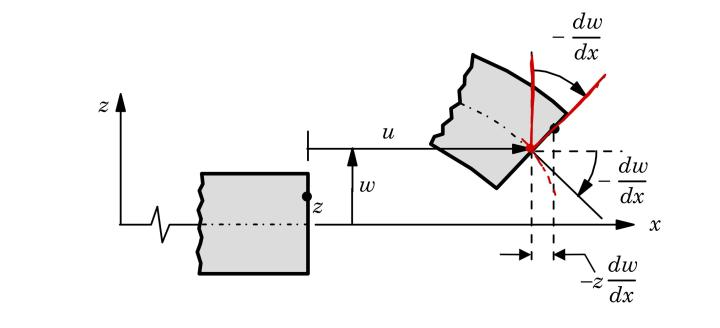
\includegraphics[width=0.7\linewidth]{Figure/fig17} 		
			\end{figure}
			The displacement is given as : $u_1 = u(x) - z\frac{d w}{d x} \qquad u_2 = 0 \qquad u_3 = w(x)$ \\
			$u_1,u_2,u_3$ is the disp of any point while $u,w$ are the disp of the centroidal axis \\
			\item So the total disp can be found from the neutral axis values. 		
			
		\end{itemize}
	\end{frame}


	\begin{frame}
		\begin{itemize}
			\item The greens theorem is
			\begin{equation}
				\begin{aligned}
					E_{ij} = \varepsilon_{ij} = \frac{1}{2}\left(\frac{\partial u_i}{\partial x_j} + \frac{\partial u_j}{\partial x_i} \right) + \frac{1}{2}\frac{\partial u_k}{\partial x_i}\frac{\partial u_k}{\partial x_j}\\
					\varepsilon_{11} = \frac{\partial u_1}{\partial x_1} + \frac{1}{2}\left[\left(\frac{\partial u_1}{\partial x_1} \right)^2 + \left(\frac{\partial u_3}{\partial x_1} \right)^2 \right]
				\end{aligned}
			\end{equation}
			\item Now the axial strains of higher orders we can igore, bu the rotation of the line perpendicular to the beam is pretty large so we have to retain it.
			\item Non-linear strains where only squares of the rotations are included are known as von Karman nonlinearity 
			\item The zero strains are $\varepsilon_{33} = \varepsilon_{13} = 0$ so only non zero strain is
			\begin{equation}
				\varepsilon_{11} = \frac{d u}{d x} - z\frac{d^2 w}{d x^2} + \frac{1}{2} \left(\frac{dw}{dx} \right)^2 
			\end{equation}
			\item  So we have two longitudinal von karman strains:
			\begin{equation}
				\varepsilon^0_{11} = \frac{d u}{d x} + \frac{1}{2} \left(\frac{dw}{dx} \right)^2  \qquad ,  \quad 
				\varepsilon^1_{11} = - z\frac{d^2 w}{d x^2} 
			\end{equation}
		\end{itemize}
	\end{frame}


	\begin{frame}{Virtual displacments : Weak form}
		\begin{itemize}
			\item The weak form can be found withou knowing the governing d.e
			\item If a body is in equilibrium, the toal virtual work done in moving through the repsective displacements is zero
			\begin{equation}
				\delta W^e = \delta W_I^e + \delta W_E^e
			\end{equation}
			$\delta W_I^e$ denotes the virtual strain stored due to the actual cauchy or second piolay stresses (Same geom) $\sigma_{ij}$\\
			$\delta W_E^e$ is the work done by external applied loads	
		\end{itemize}
	\end{frame}


	\begin{frame}
		\begin{itemize}
			\item So we have
			\begin{equation}
			\begin{aligned}
			\delta W_I^e = \int_V^e \delta \varepsilon_{xx} \sigma_{xx} dV = \int_{x_a}^{x_b} \int_A^e \left(\frac{d \delta u}{dx} + \frac{dw}{dx}\frac{d\delta w}{dx} - z \frac{d^2\delta w}{dx^2} \right) dA dx \\
			\delta W^e_E = - \left[\int_{x_a}^{x_b} q \delta w dx + \int_{x_a}^{x_b} f \delta u dx + \sum_{i=1}^{6}Q_i^e \delta \Delta_i^e \right] 
			\end{aligned}
			\end{equation}	
			\begin{figure}
				\centering
				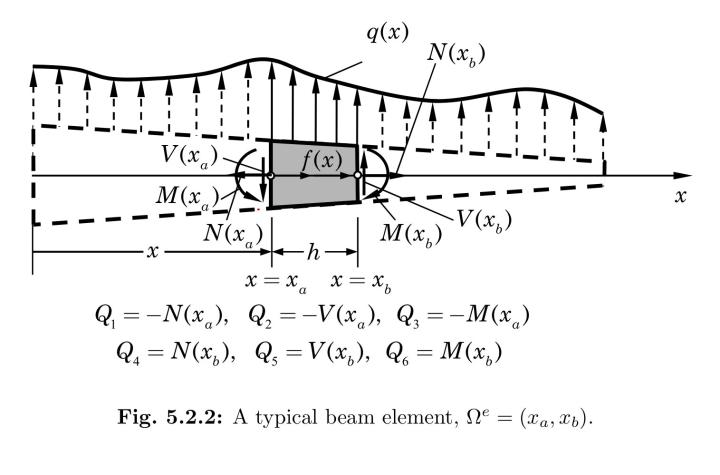
\includegraphics[width=0.7\linewidth]{Figure/fig18} 		
			\end{figure}
			
		\end{itemize}
	\end{frame}


	\begin{frame}{Sign conventions}
		\begin{figure}
			\centering
			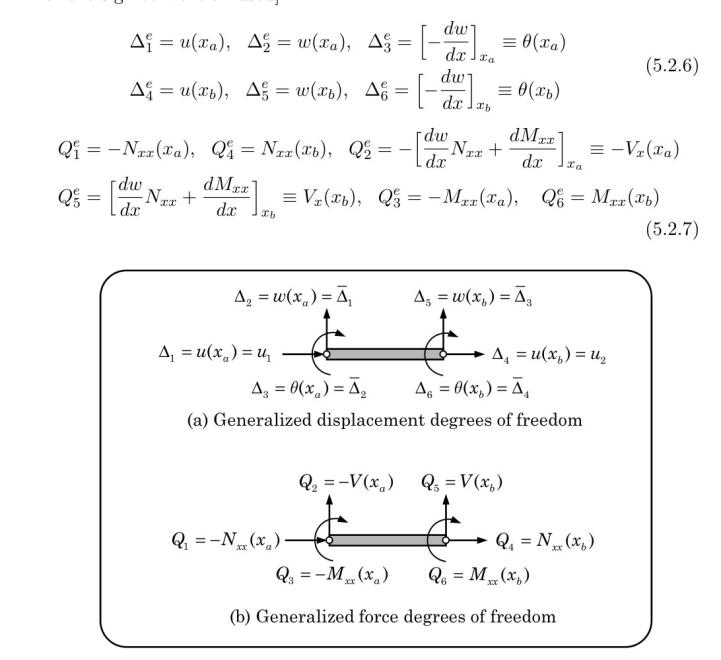
\includegraphics[width=0.6 \linewidth]{Figure/fig19} 		
		\end{figure}	
		\begin{itemize}
			\item The main thing is that for $V_x$, the component of $N_x$ is $sin(\frac{dw}{dx}) \approx \frac{dw}{dx}$, and also in moment equilibirum we get $N_{xx}\frac{dw}{dx}\Delta x = N_{xx}\Delta w$
			
		\end{itemize}
	\end{frame}


	\begin{frame}
		\begin{itemize}
			\item The free body diagram is what it is. But we can take our generalised displacement and force dof signs based on what we want.
			\item Generalised is used to show that rotationsa and moments are treated as displacements and forces
			\item By integrating in the area we get the virtual work as 
			\begin{equation}
				\delta W_I^e = \int_{x_a}^{x_b} \left[  \left(\frac{d \delta u}{dx} 
				+ \frac{dw}{dx}\frac{d\delta w}{dx} \right)N_{xx} - \frac{d^2 \delta w}{dx^2} M_{xx}\right] - \int_{x_a}^{x_b} \delta w q dx - \int_{x_a}^{x_b} \delta u f dx  - \sum_{i=1}^{6} \delta \Delta_i^e Q_i^e
			\end{equation}
			where $N_{xx} = \int_A \sigma_{xx}dA \qquad M_{xx} = \int_A \sigma_{xx}zdA$ 
		\end{itemize}
	\end{frame}


	\begin{frame}
		By taking the individual virtual terms, as the coefficients have to seperately equal to zero we get \\
		$\int_{x_a}^{x_b} \left( \frac{d\delta u}{dx}N_{xx} -\delta u f\right)dx - \delta \Delta_1^e Q_1^e - \delta \Delta_4^e Q_4^e = 0$\\
		$\int_{x_a}^{x_b} \left( \frac{d\delta w}{dx}\left(\frac{dw}{dx}N_{xx} \right) -\frac{d^2 \delta w }{dx^2}M_{xx} - \delta w q\right)dx - \delta \Delta_2^e Q_2^e - \delta \Delta_3^e Q_3^e - \delta \Delta_5^e Q_5^e -  \delta\Delta_6^e Q_6^e = 0$
		\begin{itemize}
			\item By integration by parts we get the euler lagrange equilibrium equations : given as 
			\begin{equation}
				\begin{aligned}
					\int_{x_a}^{x_b} \delta u\left( -\frac{d\delta N_{xx}}{dx} - f\right)dx - \delta \Delta_1^e Q_1^e + \left[\delta u N_{xx}\right]_{x_b}^{x_a} - \delta \Delta_4^e Q_4^e = 0\\
					\int_{x_a}^{x_b} - \delta w\left( \frac{d}{dx}\left(\frac{dw}{dx}N_{xx} \right) +\frac{d^2 M_{xx}}{dx^2} + q\right)dx - \left[ \frac{d\delta w}{dx} M_{xx}\right]_{x_b}^{x_a}  \\+  \left[ \delta w \left(\frac{dw}{dx}N_{xx} + \frac{d M_{xx}}{dx}  \right)\right]_{x_b}^{x_a} - \delta \Delta_2^e Q_2^e - \delta \Delta_3^e Q_3^e -  \delta\Delta_5^e Q_5^e -  \delta\Delta_6^e Q_6^e = 0
				\end{aligned}
			\end{equation}
		\end{itemize}
	\end{frame}


	\begin{frame}
		\begin{itemize}
			\item We get our euler equations from coefficients of the two variations
			\begin{equation}
			\begin{aligned}
				-\frac{dN_{xx}}{dx} = f(x) \\
				-\frac{d}{dx}\left(\frac{dw}{dx}N_{xx} \right) - \frac{d^2 M_{xx}}{dx^2} = q(x)
			\end{aligned}
			\end{equation}
			\item We get our boundary conditions as follows :
			\begin{equation}
			\begin{aligned}
			  Q_1^e = -N_{xx}(x_a) \qquad \qquad Q_4^e = N_{xx}(x_b) \\
			  Q_2^e = -\left[ \frac{dw}{dx}N_{xx} + \frac{dM_{xx}}{dx}\right]_{x_a} \quad 
			  Q_5^e = \left[ \frac{dw}{dx}N_{xx} + \frac{dM_{xx}}{dx}\right]_{x_b} \\
			  Q_3^e = M_{xx}(x_a) \qquad\qquad  Q_6^e = M_{xx}(x_b) \\
			\end{aligned}
			\end{equation}
			Again the - sign makes all the Qs positive in the equation
		\end{itemize}
	\end{frame}


	\begin{frame}
		\begin{itemize}
			\item We can also find the differential equations by writing the equilibirum equaitons (Fx,Fy,Mz = 0) for a small element and then take $\Delta x \rightarrow 0$. But we don't get the boundary conditions by using this. 
			\item After getting the euler lagrange differnetial equations, we can again use the weighted residual method to find the stiffness forms
			\begin{figure}
				\centering
				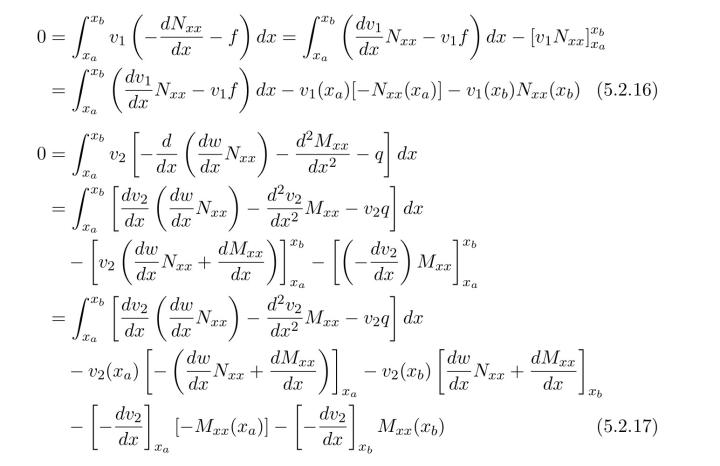
\includegraphics[width=0.8 \linewidth]{Figure/fig20} 		
			\end{figure}
			\item We clearly see that the weights are nothing but the variations and the external load work has been replaced by the internal force equivalents!!!!
		\end{itemize}
	\end{frame}


	\begin{frame}
		\begin{itemize}
			\item Now the funny thing is that we kept as N and M and now we shall replace them by 
			\begin{equation}
				\begin{aligned}
					N_{xx} = \int_A \sigma_{xx} dA = \int_{A^e} E^e \left[\frac{du}{dx} + \frac{1}{2}(\frac{dw}{dx})^2 - z\frac{d^2w}{dx^2} \right] dA \\
					= A^e \left[\frac{du}{dx} + \frac{1}{2}(\frac{dw}{dx})^2 \right] - B^e z\frac{d^2w}{dx^2}\\
					M_{xx} = \int_{A^e} \sigma_{xx} z dA = B^e  \left[\frac{du}{dx} + \frac{1}{2}(\frac{dw}{dx})^2 \right] - D^e \frac{d^2w}{dx^2}
				\end{aligned}
			\end{equation}
			where $A = EA,\qquad B = 0 \left(\int z dA = 0 \right) ,\qquad D = EI \left(\int z^2 dA \right)$
			\item Therefore the virtual work equations can be written as
			\begin{equation}
			\begin{aligned}
				0 = \int_{x_a^e}^{x_b^e} \left( A \frac{d\delta u}{x} \left[\frac{du}{dx} + \frac{1}{2}\left(\frac{dw}{dx} \right)^2 \right] -f\delta u\right) dx - \delta u(x_a)Q_1 - \delta u(x_b)Q_4 \\
				0 = \int_{x_a^e}^{x_b^e} \left( \frac{d\delta w}{dx}\frac{dw}{dx}A \left(\frac{du}{dx} + \frac{1}{2}\left(\frac{dw}{dx} \right)^2 \right) + D \frac{d^2 \delta w}{dx^2} \frac{d^2w}{dx^2} - q\delta w  \right) dx  \\ - \delta w(x_a) Q_2 - \delta \theta(x_a)Q_3 - \delta w(x_b) Q_5- \delta \theta(x_b)Q_6 
			\end{aligned}
			\end{equation}
		\end{itemize}
	\end{frame}


	\begin{frame}{FEM}
		\begin{itemize}
			\item We take the rotation as $\theta = - \frac{dw}{dx}$
			\item  We approximate the axial disp as linear lagrange and the transverse with hermite cubic interpolation functions 
		\end{itemize}
	\end{frame}


	\begin{frame}{FEM}
		\begin{figure}
			\centering
			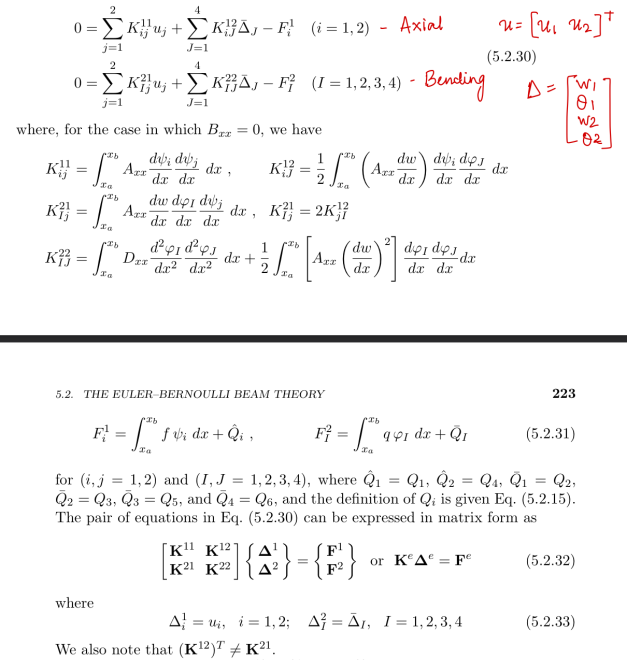
\includegraphics[width=0.66 \linewidth]{Figure/fig21} 		
		\end{figure}
	\end{frame}


	\begin{frame}
		\begin{itemize}
			\item Note that the Stiffness is not symmetric. When nonlinearity is not there then 12 and 21 (which depend on w) become 0 and the system is uncoupled. That is axial is only dependant on $u$ and bending only dependant on $\Delta$.
			\item See that we have tried to keep the shape functions symmetric
			\item When we find these conefficients from the previous iteration and then we say that the equations are linearised
			\item  The coefficients can be different if we had accounted for the terms differently, and uncouple then to a system of equations . Read reddy page 223 for this (Did not understand as of now)
			\item  We can also decompose the matrix because the 12 and 21 terms are very similar (Reddy 224)
			\item We obviously solve using direct iterative or NR method. Check reddy for the derivations of T 
		\end{itemize}
	\end{frame}


	\begin{frame}{Membrane locking}
		\small
		\begin{itemize}
			\item For the von Karman nonlinearity, for two beams : roler roler and pined pined under transverse loading. Will not have $u = 0$ because of the coupling and the solution will not be thesame. 
			\item  Suppose the roler roler beam has a constraint on u in the middle to remove rigid body movemenl, and transverse load does not make axial strain because the beam can slide without making stresses. This will have higher transverse deflection because it can stretch.
			\item The pined pined however has constraints on x = 0 and x = L so it will develop axial strains.
			\item  To make sure that the roler roler does not have any axial strain \\
			$\varepsilon_{xx}^o = \frac{du}{dx}+\frac{1}{2}(\frac{dw}{dx})^2 = 0$\\
			And basically both shoud be of the same order $-\frac{du}{dx} = \left(\frac{dw}{dx} \right)^2$
			\item So when w is cubic $\frac{dw}{dx}$ is square and the power makes it quad. So $u$ should be atleast order fifth. Taking u with any polynomial less , will make the constraint not satisfied and stiff, giving zero displacement field. (Membrane locking)
			\item We can also treat the axial strain  as constant. Since $\frac{du}{dx}$ is const, we can make $(\frac{dw}{dx})^2$ also constant. We can do this by reduced integration of all nonlinear stiffness coefficients (A,B,D).
		\end{itemize}
	\end{frame}


	\begin{frame}{Computation of stresses and strains}
		\begin{itemize}
			\item Strains and stresses are close when found at the Gauss points
			\item u is aprrox with linear lagrange and w is approx with hermite cubic polynomials.
			\item Membrane strain $\varepsilon^0_{xx}$ is assumed constant is evaluated using one point G.Q, and the bending strain $\varepsilon^1_{xx}$ is also linear and done by one point G.Q.
			\item 
			\begin{equation}
			\begin{aligned}
				\varepsilon^0_{xx} = \frac{du}{dx} + \frac{1}{2}\left(\frac{dw}{dx} \right)^w \\ 
				\varepsilon^1_{xx} = -\frac{d^2w}{dx^2}
			\end{aligned}
			\end{equation}
			And the stresses are given as follows :
			\item $\sigma_{xx} = \sigma_{xx}^0 + z\sigma_{xx}^1 = E \varepsilon_{xx}^0 + z E \varepsilon_{xx}^1$ \\
			
		\end{itemize}
	\end{frame}



	\begin{frame}{Timoshenko beam theory (TBT)}
		\begin{itemize}
			\item The euler bernoulli beam is based on fact that a straight line transverse to axis before defomration remains (1) straight (2) inextensible (3) normal to mid plane after deformation. In TBT, we say the last assumption, the rotation is independant of the slope
			\item So we get the displacement field with an independant slope
			\begin{equation}
				u_1 = u(x) + z \phi_x(x) \qquad u2 = 0 \qquad u_3 = w(x)
			\end{equation} 
			\item The non zero strains are :
			\begin{equation}
			\begin{aligned}
				\varepsilon_{xx} = \frac{du_1}{dx} + \frac{1}{2}(\frac{du_3}{dx})^2 = \frac{du}{dx} + \frac{1}{2}(\frac{dw}{dx})^2 + z \frac{d\phi}{dx} = \varepsilon^0_{xx} + z\varepsilon^1_{xx} \\
				\gamma_{xz} = \frac{du_1}{dz}  \frac{du_3}{dx} = \phi + - \left(-\frac{dw}{dx} \right) = \gamma_{xz}^0
			\end{aligned}
			\end{equation}	
			The last one we get because we remove the rotation due to w
		\end{itemize}
	\end{frame}


	\begin{frame}
		\begin{itemize}
			\item The virtual strains are :
			\begin{equation}
				\begin{aligned}
					\delta \varepsilon_{xx}^0 = \frac{d\delta u}{dx} + \frac{dw}{dx}\frac{d\delta w}{dx} \\
					\delta \varepsilon^1_{xx} = z \frac{d\phi}{dx} \\
					\delta \gamma_{xz} = \delta \phi + \frac{d \delta w}{dx} 
				\end{aligned}
			\end{equation}	
		\end{itemize}
		\begin{figure}
			\centering
			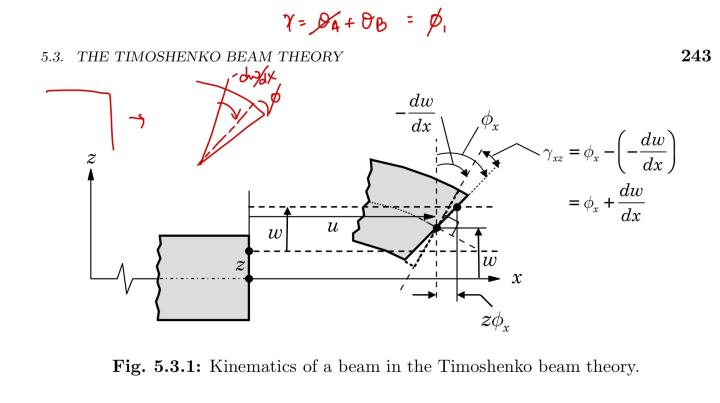
\includegraphics[width=0.66 \linewidth]{Figure/fig22} 		
		\end{figure}
	\end{frame}


	\begin{frame}{Weak form}
		\begin{itemize}
			\item The weak form is similaly developed (Reddy 243)
			\begin{equation}
			 \delta W = \int_{x_a^e}^{x_b^e} \int_{A^e} \left(N_{xx} \delta \varepsilon_{xx}^0 + M_{xx}\delta\varepsilon_{xx}^1 + Q_x \delta\varepsilon_{xz}^0 \right) - \delta W_E^e
			\end{equation}
			Note that : \\
			$N = \int \sigma dA, \quad M =  \int \sigma z dA \quad Q =  \int \sigma_{xz}dA$ \\
			$\sigma =  E\varepsilon \quad \sigma_{xz} = KG\gamma_{xz}$
			\\
			The K thing is cause we assume a constant shear over the cross section when we just say stress is G x strain. So it is a correcting factor! We compare the two energies and then we find K.
			\item Trying to keep all the variations in the same derivative order, we get the euler equilibrium equations, taking each coefficient as zero
			\begin{equation}
				\begin{aligned}
					\delta u : \quad -\frac{dN}{dx} = f(x) \\
					\delta w : \quad -\frac{dQ}{dx}  - \frac{d}{dx}\left(N \frac{dw}{dx} \right) = q(x)\\
					\delta\phi : -\frac{dM}{dx} + Q_x = 0
				\end{aligned}
			\end{equation}
			u,w, $\phi$ are the primary and N,Q,M are the secondary variables
		\end{itemize}
	\end{frame}


	\begin{frame}
		\begin{itemize}
			\item We keep the secondary variables in terms of the independant primary variables
			\begin{equation}
			\begin{aligned}
				N = A \left[ \frac{du}{dx} + \frac{1}{2} \left(\frac{dw}{dx} \right)^2\right] + B \frac{d\phi}{dx} \\
				M = B \left[ \frac{du}{dx} + \frac{1}{2} \left(\frac{dw}{dx} \right)^2\right] + D \frac{d\phi}{dx} \\
				Q = S \left(\frac{dw}{dx} + \phi \right)
			\end{aligned}
			\end{equation}
			 A,B,D are the previous terms moments of area giving the integral only in the x direction in the virtual work. S is the shear stiffness given as $S = K \int G dA = K G A =  \frac{KEA}{2(1+ \nu)}$
			 \item  Obviously we can derive the governing differential equilibrium equations (Page 245). For homogeneous beams , we have B = 0. which are the equilibrium equations given by the variational principle
		\end{itemize}
	\end{frame}


	\begin{frame}{FEM}
		\begin{itemize}
			\item The virtual work statement is then given as 
			\begin{figure}
				\centering
				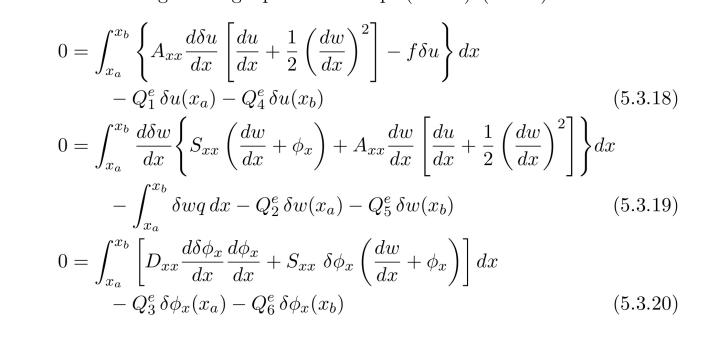
\includegraphics[width=0.8 \linewidth]{Figure/fig23} 		
			\end{figure}
			\item  The Q's have the same meaning as the euler bernoulli element
		\end{itemize}
	\end{frame}


	\begin{frame}{FEM}
		\begin{figure}
			\centering
			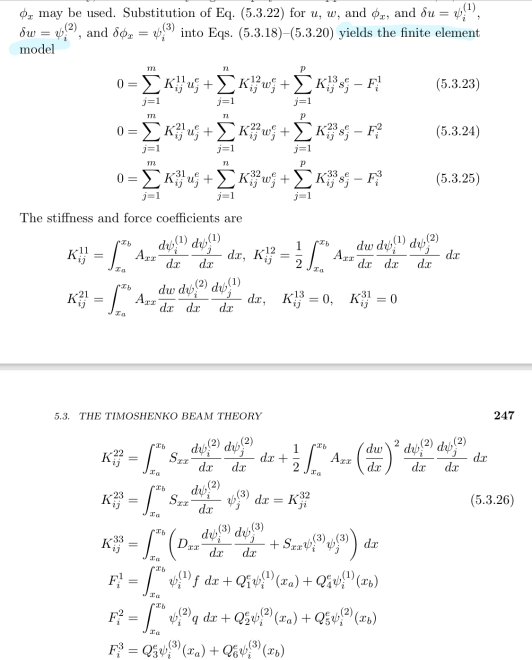
\includegraphics[width=0.5 \linewidth]{Figure/fig24} 		
		\end{figure}
		\begin{itemize}
			\item We then get $\ve{Ku = F}$ where $\ve{u = \mat{u,w,\phi}^T}$. Check Reddy 249 for T stiffness derivation
			
		\end{itemize}
	\end{frame}


	\begin{frame}{Shear and Membrane locking}
		\begin{itemize}
			\item Timoshenko beam without von Karman nonlinearity differ from each other in the choice of the approx function for w and $\phi$. Some are equal and others different
			\item Linear interpolation of both w and $\phi$ is the easisest. This makes the slope $\frac{dw}{dx}$ constant. In a think beam, as the length to thickness ratio becomes large (100), the slope would be equal to $-\phi$ which is linear instead of constant. 
			\item On the other hand a constant $\phi$ leads to zero bending energy while the transverse shear is nonzero. 
			\item  Check Reddy 248 ( Have not understood fully Locking issue)
			\item The primary variables may not be approximated by the same shape functions :
			\begin{equation}
			u(x) = N^1_iu_i \qquad w(x) = N^2_iw_i \qquad \phi(x) = N^3_i\phi_i
			\end{equation}
		\end{itemize}
	\end{frame}


	\begin{frame}{Functionally graded materials}
		Check reddy
	\end{frame}
	
	
\end{document}	
	\section{Two dimensional problems having a single variable}
	\begin{frame}{Model equation}
		\begin{itemize}
			\item Suppose we are trying to find the solution $u(x,y)$ of the following partial differential equation
			\begin{equation}
			 -\frac{d}{dx}\left(a_{xx} \frac{\partial du}{\partial dx} + a_{xy} \frac{\partial u}{\partial y} \right)
			 -\frac{d}{dy}\left(a_{yx} \frac{\partial du}{\partial dx} + a_{yy} \frac{\partial u}{\partial y} \right) + a_{00} u = f(x,y) \quad \text{in} \quad \Omega
			\end{equation}	
			The coefficients are also a function o u : eg $a_{xx} = f(x,y,u,\frac{\partial u}{\partial x }, \frac{\partial u}{\partial y})$
			\item When we descritize it with $\bar{\Omega}$ with a boundary $\bar{\Gamma}$, we get a residual given as :
			\begin{equation}
				R(u_h) = 
				-\frac{d}{dx}\left(a_{xx} \frac{\partial du_h}{\partial dx} + a_{xy} \frac{\partial u_h}{\partial y} \right)
				-\frac{d}{dy}\left(a_{yx} \frac{\partial du_h}{\partial dx} + a_{yy} \frac{\partial u_h}{\partial y} \right) + a_{00} u = f(x,y)
			\end{equation}
		\end{itemize}
	\end{frame}


	\begin{frame}{Weak form}
		The step is to multiply the residual with the ith weight function $w_i(x,y)$ which should be differentiable too. We then set $w_iR$ over the element domain $\Omega^e = 0$
		\begin{itemize}
			\item $0 = \int_{\Omega_e} w_i \left[ 
			-\frac{d}{dx}\left(a_{xx} \frac{\partial u_h}{\partial x} + a_{xy} \frac{\partial u_h}{\partial y} \right)
			-\frac{d}{dy}\left(a_{yx} \frac{\partial u_h}{\partial x} + a_{yy} \frac{\partial u_h}{\partial y} \right) + a_{00} u - f(x,y) \right] dxdy$
			\item Now we know : $\frac{d}{dx}\left(w \frac{du}{dx}\right) = w\frac{d^2u}{dx^2} + \frac{dw}{dx}\frac{du}{dx}$ \\ and $\int_A \frac{d}{dx}\left(w \frac{du}{dx} \right) dA= \int_S \left(w \frac{du}{dx} \right) dS$
			\item We get 
			\begin{equation}
			\begin{aligned}
			0 = \int_A \left[\frac{\partial w_i}{\partial x} \left(a_{xx} \frac{\partial u_h}{\partial x } + a_{xy} \frac{\partial u_h}{\partial y }\right) + 
			\int_A \frac{\partial w_i}{\partial y} \left(a_{yx} \frac{\partial u_h}{\partial x } + a_{yy} \frac{\partial u_h}{\partial y }\right) + a_{00}w_iu_h - w_if \right]dxdy \\
			- \int_S w_i \left[ \left(a_{xx} \frac{\partial u_h}{\partial x} + a_{xy} \frac{\partial u_h}{\partial y} \right)n_x + \left(a_{yx} \frac{\partial u_h}{\partial x} + a_{yy} \frac{\partial u_h}{\partial y} \right)n_y \right]dS
			\end{aligned}
			\end{equation}
			where $\ve{n = n_xe_1 + n_ye_2}$ which gives the direction consies of the boundary $\Gamma^e$. The second term can also be written as $-\int_S q_n dS$ which is the external flux normal as we move counter clockwise. 
		\end{itemize}
	\end{frame}


	\begin{frame}
		\begin{figure}
			\centering
			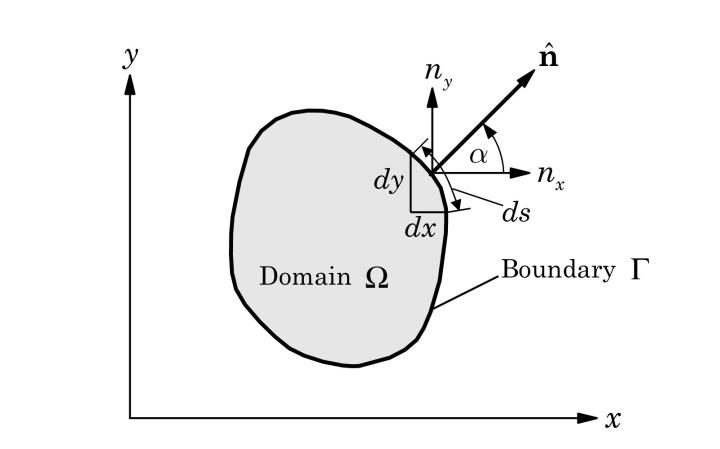
\includegraphics[width=0.5 \linewidth]{Figure/fig25} 		
		\end{figure}
	\begin{itemize}
		\item In the case of heat transfer through an anisotropic medium, aij denotes the conductivity and qn is the normal heat flux
		
	\end{itemize}
	\end{frame}


	\begin{frame}{FEM}
		\begin{itemize}
			\item The weak form states that u should be atleast linear in both x and y
			\item $u_h^e = \sum u_iN_i(x,y)$ with $N_i(x_j,y_j) = \delta_{ij} $ and $\sum_j N_j(x,y)=1$
			\begin{figure}
				\centering
				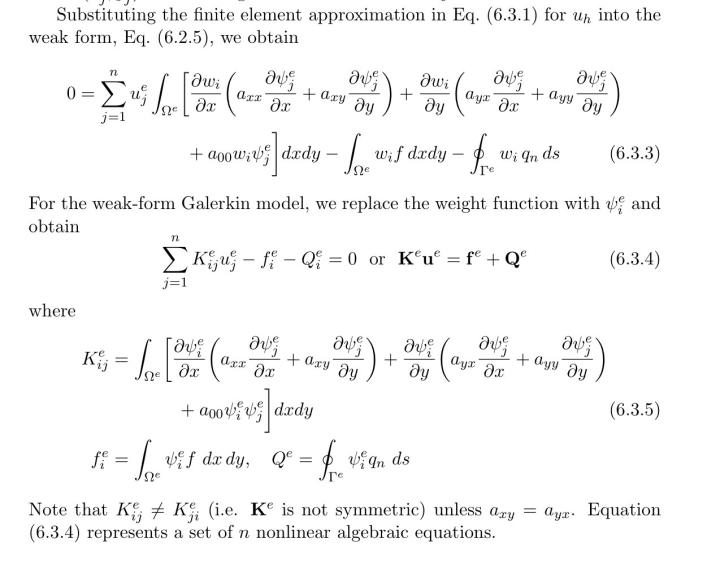
\includegraphics[width=0.8 \linewidth]{Figure/fig26} 		
			\end{figure}	
		\end{itemize}
	\end{frame}


	\begin{frame}
		\begin{itemize}
			\item The equations have to be solved by nonlinear methods
			\item The tangent T is given in page 271
		\end{itemize}
	\end{frame}


	\begin{frame}{Axisymmetric problems}
		\begin{itemize}
			\item The differential equation in cylindrical coordinate system (r,$\theta,z$)
			\begin{equation}
				-\frac{1}{r}\frac{\partial}{\partial r}\left(ra_{rr}\frac{\partial u}{\partial r} \right)
				- \frac{1}{r^2}\frac{\partial}{\partial \theta}\left(a_{\theta\theta}\frac{\partial u}{\partial \theta} \right)
				- \frac{\partial}{\partial z}\left(a_{zz}\frac{\partial u}{\partial z} \right) = f
			\end{equation} 
			\item where u,f and the coefficients are a function of (r,$\theta,z$)
			\item Dependant on the coefficents, boundary conditions and load f the problem can be made to 2D or even 1D
			\item If the cylinder is very long and stuff dont vary and depend on z, then we can assume a disk. No also if there is independance from $\theta$ then we can even just do a radial line \footnote{We just remove the derivatives in the equations where the change will be zero}
			\begin{figure}
				\centering
				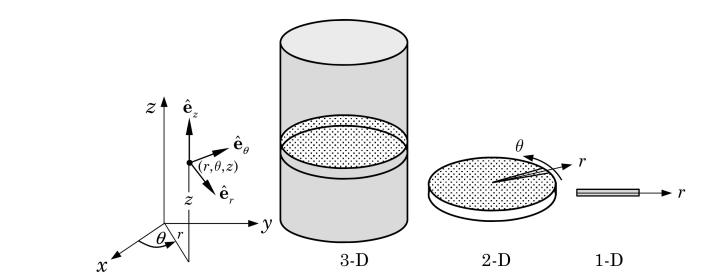
\includegraphics[width=0.8 \linewidth]{Figure/fig27} 		
			\end{figure}
		\end{itemize}
	\end{frame}


	\begin{frame}{FEM}
		\begin{itemize}
			\item Suppose all the variables are not dependant on $\theta$, therefore we would get something like a plane and the Governing differential equation will be
			\begin{equation}
				-\frac{1}{r}\frac{\partial}{\partial r}\left(ra_{rr}\frac{\partial u}{\partial r} \right)
				- \frac{\partial}{\partial z}\left(a_{zz}\frac{\partial u}{\partial z} \right) = f(r,z)
			\end{equation}
			\item The weighted statement and weak form (Using greens theorem) will be given as :
			\begin{equation}
			\begin{aligned}
			 0 = \int_A w_i \left[ 	-\frac{1}{r}\frac{\partial}{\partial r}\left(ra_{rr}\frac{\partial u}{\partial r} \right)
			 - \frac{\partial}{\partial z}\left(a_{zz}\frac{\partial u}{\partial z} \right) - f(r,z)\right] rdrdz \\
			 = \int_A \left[ a_{rr}(r,z,u_h) \frac{\partial w_i}{\partial r}\frac{\partial u_h}{\partial r}
			 + a_{zz}(r,z,u_h) \frac{\partial w_i}{\partial z} \frac{\partial u_h}{\partial z}\right] rdrdz - \int_A w_if(r,z)rdrdz - \int_S w_iq_n ds 
			\end{aligned}
			\end{equation}
			where $q_n = r\left[ a_{rr} \frac{\partial u_h}{\partial r}n_r + a_{zz}\frac{\partial u_h}{\partial z} n_z\right]$
			\item And we get $\ve{Ku = f+Q = F}$
			\item Remember the shape functions are functions of N(r,z)	
	\end{itemize}
	\end{frame}


	\begin{frame}{Numerical integration}
		\begin{itemize}
			\item
			\begin{figure}
				\centering
				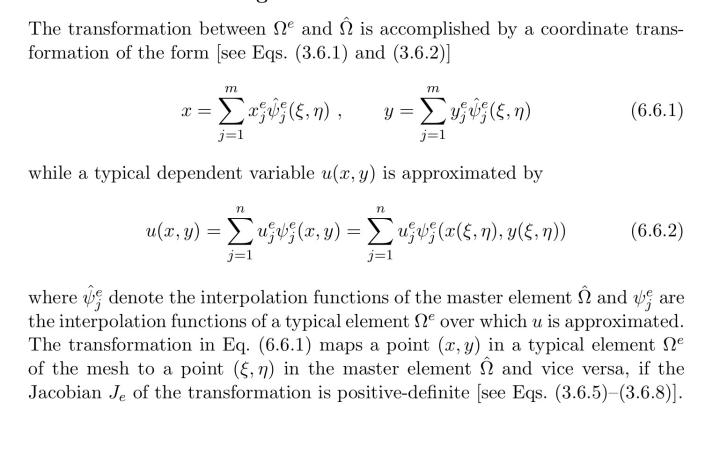
\includegraphics[width=0.9 \linewidth]{Figure/fig28} 		
			\end{figure} 
			
		\end{itemize}
	\end{frame}

	
	\begin{frame}{Gauss quad - coordinate change}
		\begin{itemize}
			\item Remember that we have to we have to transform the integral domain to the master element so that Gauss quadrature can be usd. The derivatives in the original geometry are also expressed with respect to $\xi,\eta$ given by
			\begin{equation}
			\mat{\frac{\partial N_i}{\partial dx}; ;\frac{\partial N_i}{\partial dy} } = \ve{J^{-1}} \mat{\frac{\partial N_i}{\partial d\xi}; ;\frac{\partial N_i}{\partial d\eta} } 
			\end{equation}
			where $\ve{J} = \mat{\frac{\partial x}{\partial \xi}, \frac{\partial y}{\partial \xi}; , ; \frac{\partial x}{\partial \eta}, \frac{\partial y}{\partial \eta}} =
			\mat {\sum x_i \frac{\partial N_i}{\partial \xi}, \sum y_i \frac{\partial N_i}{\partial \xi} ; , ; 
			\sum x_i \frac{\partial N_i}{\partial \eta}, \sum y_i \frac{\partial N_i}{\partial \eta}} = \mat{\frac{\partial N_1}{\partial \xi}, \frac{\partial N_2}{\partial \xi}, .... ,\frac{\partial N_m}{\partial \xi} ; , , ,;
			\frac{\partial N_1}{\partial \eta}, \frac{\partial N_2}{\partial \eta}, ...., \frac{\partial N_m}{\partial \eta} }
	 		\mat{x_1, y_1; , ; x_2, y_2; , ; \vdots, \vdots; x_m,y_m}$ 
	 		\item If the same shape functionsa re used for the geometry and field variable, we say its isoparametric
		\end{itemize}
	\end{frame}


	\begin{frame}
		\begin{figure}
			\centering
			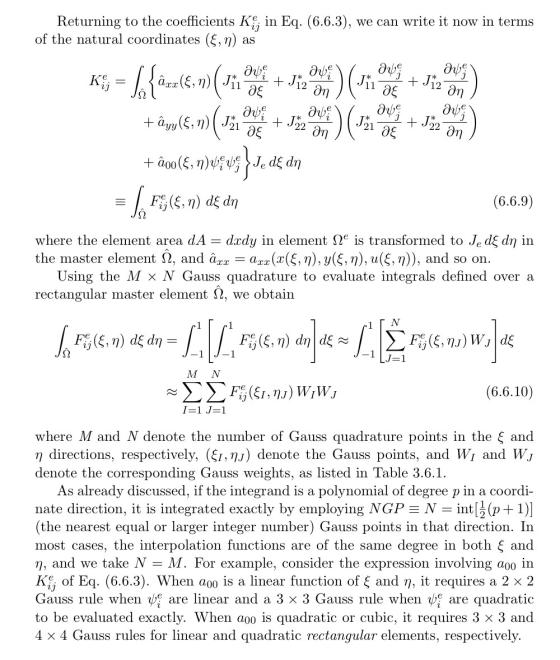
\includegraphics[width=0.6 \linewidth]{Figure/fig29} 		
		\end{figure} 
	where J* are the components of the inverse jacobian
	\end{frame}


	\section{Time dependant problems}
	
	\begin{frame}{Time dependacy}
		Will have to read later!!
	\end{frame}



\section{Plates}

	\begin{frame}
		\begin{itemize}
			\item Plate has large dimension compared to thickness. No need to use 3D, with study the deformations and stresses in plates, smal rotations and large displacement (w/h>1)
			\item Extension of Euler berunoulli is called Kirchoff plate. Extension of timoshenko beam is the first order or mindlin shear deformation plate theory.
			\item $\ve{X}$ is used for the material coordinates and $\ve{x}$ is used for the spatial coordinates. No distinction is made between the material and spatial coordinates. 	
		\end{itemize}
	\end{frame}


	\begin{frame}{Classical plate theory}
		The disp satisfy the kirchoff rules which are an extension of the euler bernoulli hypothesis which are
		\begin{itemize}
			\item Straight lines perpendicular to the mid surface remain straight
			\item Transverse normals do not have elongation
			\item Cross sections remain perpendiuclar under rotation
		\end{itemize}
	\end{frame}


	\begin{frame}{Dislacement and strain fields}
		\begin{itemize}
			\item We have the domain of the plate as $\Omega_o \times (-h/2,h/2)$. The boundary of the top surface $z = h/2$ and bottom surface $z = -h/2$ with boundary $\Gamma$ which is a curved surface with outward normal $\ve{n} = n_xe_1 + n_ye_2$
			\begin{figure}
				\centering
				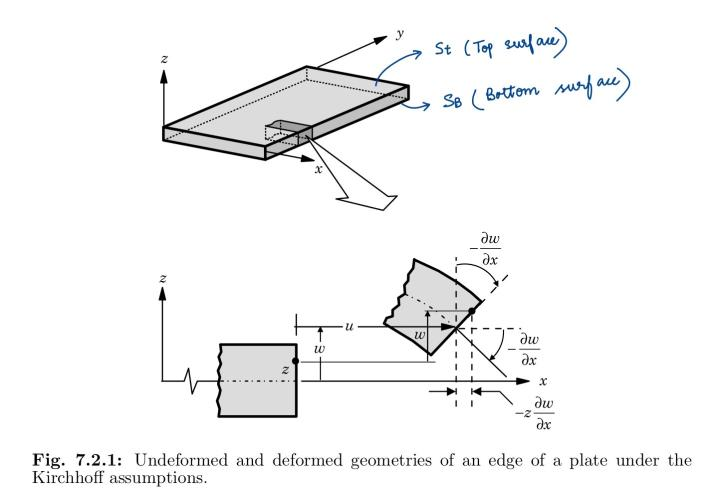
\includegraphics[width=0.8 \linewidth]{Figure/fig30} 		
			\end{figure}
		\end{itemize}
	\end{frame}


	\begin{frame}
		\begin{itemize}
			\item The kirchoff hypotehesis implies the following displacement field 
			\begin{equation}
			\begin{aligned}
				u_1(x,y,z,t) = u(x,y,t) - z\frac{\partial w}{\partial x} \\
				u_2(x,y,z,t) = v(x,y,t) - z\frac{\partial w}{\partial y} \\
				u_3(x,y,z,t) = w(x,y,t) 
			\end{aligned}
			\end{equation}
			\item Where $u,v,w$ denote the material point in the undeformed of the nerutral axis wherees $u_1,u_2,u_3$ denote any aribitary point location
			\item The componenets of the Green-Lagrange strain tensor $\ve{E}$ in terms of components of the total displacement vector $u = x(x,t) - X$ (x and X here are the same) is
			\begin{equation}
				\tiny
				\begin{aligned}
					E_{11} = \frac{\partial u_1}{\partial X_1} + \frac{1}{2}\left[ \left(\frac{\partial u_1}{\partial X_1} \right)^2 +
					\left(\frac{\partial u_2}{\partial X_1} \right)^2 + 
					\left(\frac{\partial u_3}{\partial X_1} \right)^2 \right] \\ 
					E_{22} = \frac{\partial u_2}{\partial X_2} + \frac{1}{2}\left[ \left(\frac{\partial u_1}{\partial X_2} \right)^2 +
					\left(\frac{\partial u_2}{\partial X_2} \right)^2 + 
					\left(\frac{\partial u_3}{\partial X_2} \right)^2 \right]\\
					E_{33} = \frac{\partial u_3}{\partial X_3} + \frac{1}{2}\left[ \left(\frac{\partial u_1}{\partial X_3} \right)^2 +
					\left(\frac{\partial u_2}{\partial X_3} \right)^2 + 
					\left(\frac{\partial u_3}{\partial X_3} \right)^2 \right]\\
					E_{12} = \frac{1}{2}\left[ \frac{\partial u_1}{\partial X_2} + \frac{\partial u_2}{\partial X_1} + 
					\frac{\partial u_1}{\partial X_1}\frac{\partial u_1}{\partial X_2} +
					\frac{\partial u_2}{\partial X_1}\frac{\partial u_2}{\partial X_2} +
					\frac{\partial u_3}{\partial X_1}\frac{\partial u_3}{\partial X_2} +
					\right]	\\
					E_{13} = \frac{1}{2}\left[ \frac{\partial u_1}{\partial X_3} + \frac{\partial u_3}{\partial X_1} + 
					\frac{\partial u_1}{\partial X_1}\frac{\partial u_1}{\partial X_3} +
					\frac{\partial u_2}{\partial X_1}\frac{\partial u_2}{\partial X_3} +
					\frac{\partial u_3}{\partial X_1}\frac{\partial u_3}{\partial X_3} +
					\right]	\\
					E_{23} = \frac{1}{2}\left[ \frac{\partial u_2}{\partial X_3} + \frac{\partial u_3}{\partial X_2} + 
					\frac{\partial u_1}{\partial X_2}\frac{\partial u_1}{\partial X_3} +
					\frac{\partial u_2}{\partial X_2}\frac{\partial u_2}{\partial X_3} +
					\frac{\partial u_3}{\partial X_2}\frac{\partial u_3}{\partial X_3} +
					\right]	
				\end{aligned}
			\end{equation}
		\end{itemize}
	\end{frame}


	\begin{frame}
		\begin{itemize}
			\item If the components of the displacement gradient are very small = O($\epsilon$), then the terms having O($\epsilon^2$) can be omitted in the strains. However if the rotations of the transverse normals are moderate (10 -15 degrees), then the following strains are small but not negligible
			\begin{equation}
			\left(\frac{\partial u_3}{\partial X_1} \right)^2 \qquad
			\left(\frac{\partial u_3}{\partial X_2} \right)^2 \qquad
			\frac{\partial u_3}{\partial X_1}\frac{\partial u_3}{\partial X_2}  
			\end{equation}
			\item  Thus the strains take the following (Remember that $E = \varepsilon$ where we say its small strain but moderate rotations)
			\begin{equation}
			\tiny
			\begin{aligned}
			E_{11} = \varepsilon_{11}= \frac{\partial u_1}{\partial x} + \frac{1}{2}\left[ \left(\frac{\partial u_3}{\partial x} \right)^2 \right] \qquad
			E_{22} = \frac{\partial u_2}{\partial y} + \frac{1}{2}\left[ 
			\left(\frac{\partial u_3}{\partial y} \right)^2 \right]\\
			E_{33} = \frac{\partial u_3}{\partial z} \qquad
			E_{12} = \frac{1}{2}\left[ \frac{\partial u_1}{\partial y} + \frac{\partial u_2}{\partial x} + 
			\frac{\partial u_3}{\partial x}\frac{\partial u_3}{\partial y} 
			\right]	\\
			E_{13} = \frac{1}{2}\left[ \frac{\partial u_1}{\partial z} + \frac{\partial u_3}{\partial x} 
			\right]	\qquad
			E_{23} = \frac{1}{2}\left[ \frac{\partial u_2}{\partial z} + \frac{\partial u_3}{\partial y}
			\right]	
			\end{aligned}
			\end{equation}
		\end{itemize}
	\end{frame}


	\begin{frame}
		\begin{itemize}
			\item  For this displacement field, we have $\varepsilon_{z} = \frac{\partial u_3}{\partial z} = \frac{\partial w}{\partial z} = 0$ and taking the displacement fields. The strains then reduce to
			\begin{equation}
				\begin{aligned}
				\varepsilon_{xx}= \frac{\partial u}{\partial x} + \frac{1}{2}\left[ \left(\frac{\partial w}{\partial x} \right)^2 - z \frac{\partial^2 w}{\partial x^2}\right] \qquad
				\varepsilon_{yy} = \frac{\partial v}{\partial y} + \frac{1}{2}\left[ 
				\left(\frac{\partial w}{\partial y} \right)^2 - z\frac{\partial^2 w}{\partial y^2}\right]\\
				2\varepsilon_{xy} = \gamma_{xy} = \frac{\partial u}{\partial y} + \frac{\partial v}{\partial x} + 
				\frac{\partial w}{\partial x}\frac{\partial w}{\partial y} -2z\frac{\partial^2 w}{\partial x \partial y}	\\
				2\varepsilon_{xz} = -  \frac{\partial w}{\partial x} + \frac{\partial w}{\partial x} = 0\qquad
				2\varepsilon_{yz} = - \frac{\partial w}{\partial y} + \frac{\partial w}{\partial y} = 0
				\end{aligned}
			\end{equation}
			\item These are called von Karman strains and called classical plate theory with von karman strains. Note that the transverse strains are zero in the classical plate theory. The total strains can be written as membrane + bending strain
			\begin{equation}
			\mat{\varepsilon_{xx};\varepsilon_{yy};\gamma_{xy}} =  \mat{\varepsilon_{xx}^0;\varepsilon_{yy}^0;\gamma_{xy}^0} + z\mat{\varepsilon_{xx}^1;\varepsilon_{yy}^1;\gamma_{xy}^1}
			\end{equation}
		\end{itemize}
	\end{frame}


	\begin{frame}
		\begin{itemize}
			\item The strains are expanded as : 
			\begin{equation}
			\begin{aligned}
			\mat{\varepsilon_{xx}^0;\varepsilon_{yy}^0;\gamma_{xy}^0} = 
			\mat{\frac{\partial u}{\partial x} + \frac{1}{2} \left(\frac{\partial w}{\partial x} \right)^2 ; ;
				 \frac{\partial v}{\partial y} + \frac{1}{2}\left(\frac{\partial w}{\partial y} \right)^2; ;
				\frac{\partial u}{\partial y} + \frac{\partial v}{\partial x} + 
				\frac{\partial w}{\partial x}\frac{\partial w}{\partial y} }\qquad
			\mat{\varepsilon_{xx}^1;\varepsilon_{yy}^1;\gamma_{xy}^1} = - \mat{
			\frac{\partial^2 w}{\partial x^2};; \frac{\partial^2 w}{\partial y^2};; 2\frac{\partial^2 w}{\partial x \partial y}	}
			\end{aligned}
			\end{equation}
		\end{itemize}
	\end{frame}


	\begin{frame}{Weak form of classical plate theory}
		\begin{itemize}
			\item Virtual work statement is used again to derive (Just like 4 beams). We account for thermal effects, where the material does not change with tempearture which is knowon as a fuction of the position  hence ($\delta T = 0$), so temperature eneters throught the constitutive relations.
			\item Suppose the domain is represented by fem $\Omega_e$ with  distributed transverse loads $q(x,y)$ at the top. $(\sigma_{nn},\sigma_{ns},\sigma_{nz})$ are the stress components on the boundary of the plate
			\begin{figure}
				\centering
				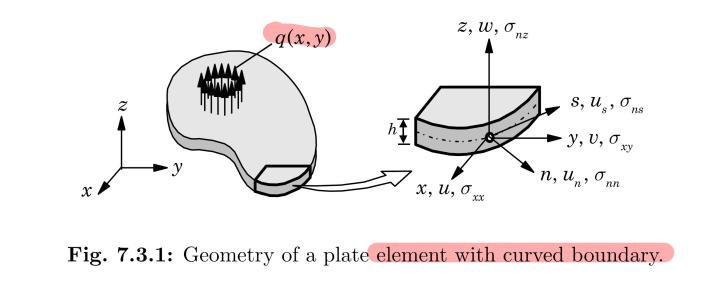
\includegraphics[width=0.8 \linewidth]{Figure/fig31} 		
			\end{figure}
		\end{itemize}
	\end{frame}


	\begin{frame}
		\begin{itemize}
			\item The principle of virtual work states that $0 = \delta W^e = \delta W_I^e + \delta W_E^e$
			\item As noted earlier, the transverse shears $\gamma_{xz},\gamma_{yz},\varepsilon_{zz}$ are zero. Therefore the transverse stresses ($\sigma_{xz},\sigma_{yz},\sigma_{zz}$ ) do not eneter the formulatin because the strains due to these are zero. Even though they are not accounted, in reality they exist to maintain equilibirum, these components can also be specified at the boudary. So they have to be accounted in the equilibirum equations. 
			\item The internal virtual strain is then given as 
			\begin{equation}
				\begin{aligned}
					\delta W_I^e = \int_A \int_{-\frac{h}{2}}^{\frac{h}{2}} 
					\left(
					\sigma_{xx} \delta \varepsilon_{xx} + \sigma_{yy} \delta \varepsilon_{yy} + 2\sigma_{xy} \delta \varepsilon_{xy}
					\right) dz~dx~dy\\
					= \int_A \left(N_{xx}\delta \varepsilon_{xx}^0 + M_{xx}\delta\varepsilon_{xx}^1 + N_{yy}\delta\varepsilon_{yy}^0 + M_{yy}\delta\varepsilon_{yy}^1 
					 + N_{xy}\delta\gamma_{xy}^0 + M_{xy}\delta\gamma_{xy}^1 \right) dx~dy
				\end{aligned}
			\end{equation}
			where N and M are the axial and the moment internal forces per unit length. 
		\end{itemize}
	\end{frame}


	\begin{frame}{Plate: Internal forces}
		\begin{figure}
			\centering
			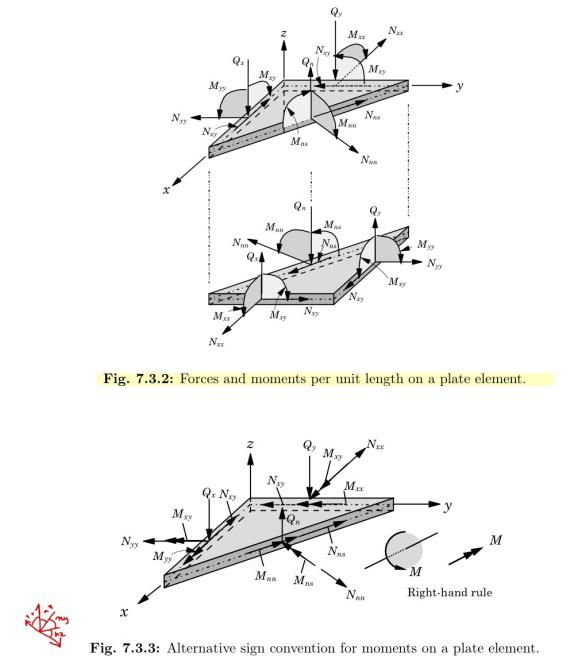
\includegraphics[width=0.6 \linewidth]{Figure/fig32} 		
		\end{figure}
	\end{frame}


	\begin{frame}
		\begin{itemize}
			\item The virtual work by the distributed transverse load q(x,y), reaction force of an elastic foundation, in plane normal stress $\sigma_{nn}$, in plane tangential stress $\sigma_{ns}$, transverse shear stress $\sigma_{nz}$ is 
			\begin{equation}
			\begin{aligned}
				\delta W_E^e = - (\int_A q(x,y) \delta w(x,y,\frac{h}{2}) dx~dy + 
				\int_A F_s(x,y) \delta w(x,y,-\frac{h}{2}) dx~dy
				\\	+ \int_S \int_{-\frac{h}{2}}^{\frac{h}{2}} \left[ \sigma_{nn} \left(\delta u_n - z \frac{\delta w}{n} \right) + \sigma_{ns} \left(\delta u_s - z \frac{\delta w}{s}\right) 
				+ \sigma_{nz}\delta w\right] dz~ds ) \\ 
				= - \left[ \int_S \left(N_{nn}\delta u_n - M_{nn}\frac{\partial \delta w}{\partial n}
							+ N_{ns}\delta u_s 
				            - M_{ns}\frac{\partial \delta w}{\partial s} + Q_n \delta w \right)ds
				            + \int_A (q-kw)\delta w dx~dy
				 \right] 
			\end{aligned}
			\end{equation}
			\item where Fs = -kw ( Foundation force), the negative sign it is the force applied upwards, but you can think of it like the potential increases as the w increases.
			\item The last term in the work term is the virtual work of the transverse and normal forces on a boundary that is inclined. Where N = $\int_{-\frac{h}{2}}^{\frac{h}{2}}\sigma$ ,  M = $\int_{-\frac{h}{2}}^{\frac{h}{2}}z\sigma$, $Q_n = \int_{-\frac{h}{2}}^{\frac{h}{2}}\sigma_{nz}$ 
		\end{itemize}
	\end{frame}


	\begin{frame}
	\begin{itemize}
		\item We now relate the stresses in the direction in the boundary to the internal stresses given in cartesion using stress tensor coordinate transformation
			\begin{equation}
			   \mat{\sigma_{nn}; \sigma_{ns}} = \mat{n_x^2,n_y^2,2n_xn_y ; -n_xn_y,n_xn_y,n_x^2 - n_y^2} \mat{\sigma_{xx};\sigma_{yy};\sigma_{xy}}
			\end{equation}
	\end{itemize}
	\end{frame}


	\begin{frame}{Weak forms}
		\begin{itemize}
			\item Keeping the weak forms in the full virtual work statement we get
			\begin{equation}
			\tiny
				\begin{aligned}
					0 =  \int_A \left(N_{xx}\delta \varepsilon_{xx}^0 + M_{xx}\delta\varepsilon_{xx}^1 + N_{yy}\delta\varepsilon_{yy}^0 + M_{yy}\delta\varepsilon_{yy}^1 
					+ N_{xy}\delta\gamma_{xy}^0 + M_{xy}\delta\gamma_{xy}^1 \right) dx~dy \\ - \left[ \int_S \left(N_{nn}\delta u_n - M_{nn}\frac{\partial \delta w}{\partial n}
					+ N_{ns}\delta u_s 
					- M_{ns}\frac{\partial \delta w}{\partial s} + Q_n \delta w \right)ds
					+ \int_A (q-kw)\delta w dx~dy
					\right]  \\ 
					 =  \int_A \left(N_{xx}\delta \varepsilon_{xx}^0 + M_{xx}\delta\varepsilon_{xx}^1 + N_{yy}\delta\varepsilon_{yy}^0 + M_{yy}\delta\varepsilon_{yy}^1 
					 + N_{xy}\delta\gamma_{xy}^0 + M_{xy}\delta\gamma_{xy}^1 \right) dx~dy \\ - \left[ \int_S \left(N_{nn}\delta u_n - M_{nn}\frac{\partial \delta w}{\partial n}
					 + N_{ns}\delta u_s 
					 - M_{ns}\frac{\partial \delta w}{\partial s} + Q_n \delta w \right)ds
					 + \int_A (q-kw)\delta w dx~dy
					 \right]  
				\end{aligned}
			\footnote{\tiny In the last three statements, It seems the equation has been kept according to the variation but how do you account for $ \delta u_n \quad \delta u_s$ as they will have components in both. Maybe the euler equations will make sense}
			\end{equation}
			
			\begin{figure}
				\centering
				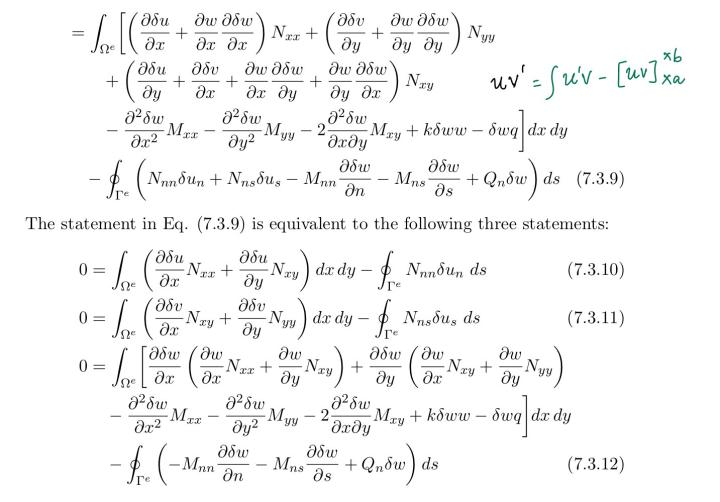
\includegraphics[width=0.6 \linewidth]{Figure/fig33} 		
			\end{figure}
	
		\end{itemize}
	\end{frame}


	\begin{frame}{Equilibrium equations}
		\begin{itemize}
			\item Keeping the virtual parameters in the same order to get the euler equations we get
			\begin{equation}
			\tiny
			\begin{aligned}
				0 = \int_A \left[ -\left(N_{xx,x} + N_{xy,y}\right)\delta u - \left( N_{xy,x} + N_{yy,y}\right)\delta v
		  			- \left(M_{xx,xx} + 2M_{xy,xy} + M_{yy,yy} + \mathcal{N} - kw + q\right) \delta w
							\right] dx~dy \\
				+ \int_S  (\left(N_{xx}n_x + N_{xy}n_y \right)\delta u  
			  + \left(N_{xy}n_x + N_{yy}n_y \right)\delta v
			  + \left( M_{xx,x}n_x + M_{xy,y}n_x + M_{yy,y}n_y + M_{xy,x}n_y + \mathcal{P} \right) \delta w \\
			  - \left(M_{xx}n_x + M_{xy}n_x \right)\frac{\partial \delta w}{\partial x} 
			  -\left(M_{xy}n_x + M_{yy}n_y \right)\frac{\partial \delta w}{\partial y} )ds  
			  -\int_S \left(N_{nn} \delta u_n + N_{ns}\delta u_s - M_{nn}\frac{\partial \delta w}{\partial n} - M_{ns}\frac{\partial \delta w}{\partial s} + Q_n \delta w \right)ds
			\end{aligned}
			\end{equation}
			\item Where 
				\begin{equation}
				\tiny
					\begin{aligned}
					\mathcal{N} = \frac{\partial }{\partial x} \left(N_{xx}\frac{\partial w}{\partial dx}   + N_{xy}\frac{\partial w}{\partial dy}\right)
					 + \frac{\partial }{\partial y} \left(N_{xy}\frac{\partial w}{\partial x} 
					+ N_{yy}\frac{\partial w}{\partial y}\right) \\
					\mathcal{P} = \left(N_{xx}\frac{\partial w}{\partial x}   + N_{xy}\frac{\partial w}{\partial y}\right) n_x
					+ \frac{\partial }{\partial y} \left(N_{xy}\frac{\partial w}{\partial x} 
					+ N_{yy}\frac{\partial w}{\partial y}\right) n_y 
					\end{aligned}
				\end{equation}
		\end{itemize}
	\end{frame}


	\begin{frame}
		\begin{figure}
			\centering
			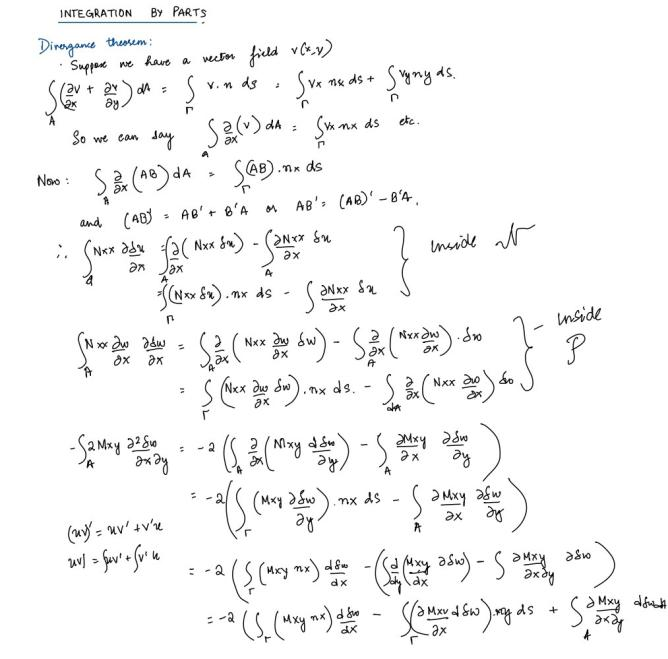
\includegraphics[width=0.7 \linewidth]{Figure/fig34} 		
		\end{figure}
	\end{frame}


	\begin{frame}{Euler-lagrange equilibrium equations}
		\begin{itemize}
			\item Keeping the coefficients of the variations (seting $\delta u, \delta v, \delta w = 0$)we get the equilibirum equations given as
			\begin{equation}
			\begin{aligned}
				\delta u : \frac{\partial N_{xx}}{\partial x} + \frac{\partial N_{xy}}{\partial y} = 0\\
				\delta v : \frac{\partial N_{xy}}{\partial x} + \frac{\partial N_{yy}}{\partial y} = 0\\
				\delta w : \frac{\partial^2 M_{xx}}{\partial x^2} + 2\frac{\partial^2 M_{xy}}{\partial x \partial y} + \frac{\partial^2 M_{yy}}{\partial y^2} + \mathcal{N} - kw + q = 0
			\end{aligned}
			\end{equation}
		\end{itemize}
	\end{frame}


	\begin{frame}{Boudnary conditions}
		\begin{itemize}
			\item To cast the B.C. on an edge whose normal is $\ve{n}$, we express the generalised displacements ($u,v,w,\frac{\partial w}{\partial x}, \frac{\partial w}{\partial y}$) in x,y,z system in the corresponding displacements in normal, tangential and transverse directions. We get
			\begin{equation}
			\begin{aligned}
				u = u_nn_x - u_sn_y \qquad v = u_nn_y + u_sn_x \\ 
				\frac{\partial w}{\partial x} = \frac{\partial w}{\partial n} n_x 
				- \frac{\partial w}{\partial s}n_y \qquad 
				\frac{\partial w}{\partial y} = \frac{\partial w}{\partial n}n_y
				+ \frac{\partial w}{\partial s}n_x
			\end{aligned}
			\end{equation}
			\begin{figure}
				\centering
				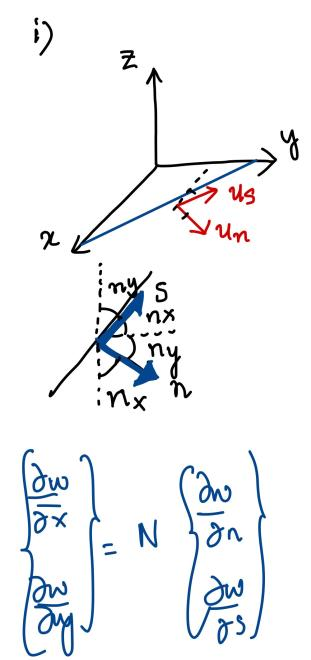
\includegraphics[width=0.2  \linewidth]{Figure/fig35} 		
			\end{figure}
		Now the derivative of $w$ is a vector which can undergo basis transformation
 		\end{itemize}
	\end{frame}


	\begin{frame}{Boundary conditions}
		\begin{itemize}
			\item The boundary conditions can be written in the normal, tangenetial coords 
			\begin{equation}
			\tiny
			\begin{aligned}
			\int_S [ 
			\left(N_{xx}n_x + N_{xy}n_y\right)\left(\delta u_nn_x - \delta u_sn_y\right) +
			\left(N_{xy}n_x + N_{yy}n_y\right)\left(\delta u_nn_y + \delta u_sn_x\right) \\ +
			\left( M_{xx,x}n_x + M_{xy,y}n_x + M_{yy,y}n_y + M_{xy,x}n_y + \mathcal{P} \right) \delta w \\ - 
			\left(M_{xx}n_x + M_{xy}n_y \right)\left(\frac{\partial w}{\partial n} n_x 
			- \frac{\partial w}{\partial s}n_y \right) - 
			\left(M_{xy}n_x + M_{yy}n_y \right)\left(\frac{\partial w}{\partial n} n_y 
			+ \frac{\partial w}{\partial s}n_x \right)]ds\\
			 - \int_S \left(N_{nn} \delta u_n + N_{ns}\delta u_s - M_{nn}\frac{\partial \delta w}{\partial n} - M_{ns}\frac{\partial \delta w}{\partial s} + Q_n \delta w \right)ds
			\end{aligned} 
			\end{equation}
			\item $\delta u$ in natural does not change the direction cosines because here they are constant dependant on the geometry we are at and not the variation.
		\end{itemize}
	\end{frame}


	\begin{frame}{Boundary conditions}
		\begin{figure}
			\centering
			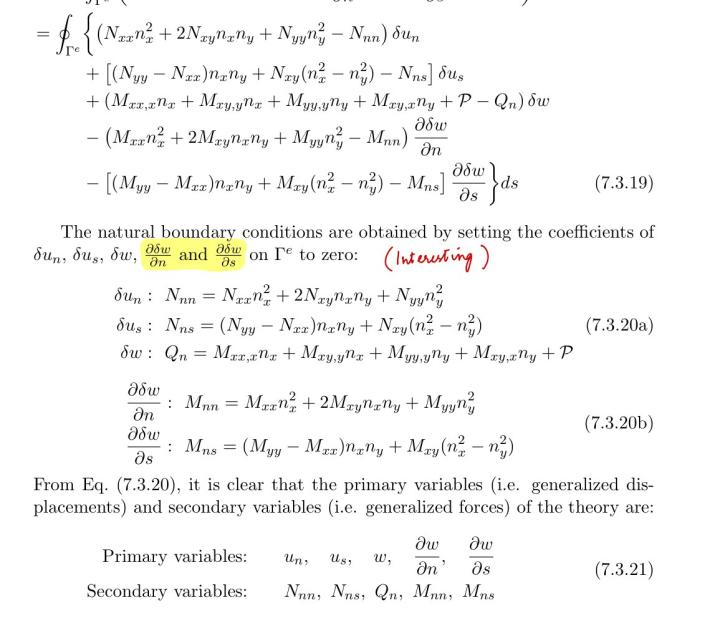
\includegraphics[width=0.7\linewidth]{Figure/fig36} 		
		\end{figure}
		\begin{itemize}
			\tiny
			\item I find this interesting to keep the varitaion with derivatives equal to zero.
			\item We see that from the equilibrium equations, if we keep them in displacements we woul get a DE having second order spatial derivatives of u, v and fourth order of w. Therefore we need eight boundary conditions (4 primary and 4 natural). But we have eight
		\end{itemize}
	\end{frame}


	\begin{frame}{Kirchoff free-edge condition}
		\begin{itemize}
			\item To remove this problem, one can integrate the tangential derivative term by parts
			\begin{equation}
				-\int_S M_{ns}\frac{\partial \delta w}{\partial s} ds = \int_S \frac{\partial M_{ns}}{\partial s}\delta w ds - [M_{ns}\delta w]_{\Gamma}
			\end{equation}
			\item The second term [$M_{ns}\delta w$] is zero when the end points of two curves meet or when $M_{ns} = 0$. If $M_{ns}$ is not specified at the corners, then concentrated forces $F = -2M_{ns}$ are produced at the corners. 2 appears from the two sides of the corner. 
			\item The remaining boundary term is added to the shear force $Q_n$ (Also having a coefficien of $\delta w$ in integral  S)to get
			\begin{equation}
				V_n = Q_n + \frac{\partial M_{ns}}{\partial s}
			\end{equation}
			This specification of theshare force is known a sthe Kirchoff free edge condition. The final boundary conditions are 
			\begin{equation}
			\begin{aligned}
			\text{Genearlised dispalcements} : u_n, u_s,w,\frac{\partial w}{\partial n} \\
			\text{Generalised forces} : N_{nn}, N_{ns}, V_n, M_{nn}
			\end{aligned}
			\end{equation}
			\footnote{So you known either one he displacement of the forces. On a side parallel to x asix (s = x and n =y). $u_n =v, u_s = u, w, \frac{\partial w}{\partial n} = \frac{\partial w}{\partial y}, N_{nn}=N_{yy},N_{ns}=N_{yx}, V_n =V_y,M_{nn}=M_{yy}$}
		\end{itemize}
	\end{frame}


	\begin{frame}{Typical edge conditions}
		We discuss for some common boundary with edges parallel to x and y coordinates
		\begin{itemize}
			\item \textbf{Free edge with normal $\ve{n}$} : We don't know the disp but we know the force/moment
			\begin{equation}
				\begin{aligned}
				u_n \neq 0, \quad u_s \neq 0, \quad w \neq 0, \quad \frac{\partial w}{\partial n} \neq 0 \\
				N_{nn} = \hat{N_{nn}}, \quad N_{ns} = \hat{N_{ns}}, V_n =  Q_n + \frac{\partial M_{ns}}{\partial s} = \hat{V_n}, M_{nn} = \hat{M_{nn}}
				\end{aligned}
			\end{equation}
			\item \textbf{Fixed with normal $\ve{n}$} : Fixed edge with primary values known. But we dont know the reaction forces and moments. Given as \\
			$u_n =0, \quad u_s =0,\quad w = 0,\quad \frac{\partial w}{\partial n} = 0 $. 
			\item \textbf{Simply suppored} : This is not unize especially when both inplane and bending are coupled. Here showing two types
			\begin{enumerate}
				\item SS1: $u_s = 0, \quad w =0 \quad, N_{nn}=\hat{N_{nn}}, \quad M_{nn} = \hat{M_{nn}}$
				\item SS2: $u_n = 0, \quad w =0 \quad, N_{ns}=\hat{N_{ns}}, \quad M_{nn} = \hat{M_{nn}}$
			\end{enumerate}
			
		\end{itemize}
	\end{frame}


	\begin{frame}{Stress resultant-Deflection relations}
		\begin{itemize}
			\item To express the foces and moments (N,M) per unit length in terms of the generalized displacements we need to bring the correct stress-strain relations. In the classical plate theory all the transverse strain components ($\varepsilon_{xx,xz,yz}$) are zero.
			\item  Since $\varepsilon_{zz} = 0$, the transverse normal stress $\sigma_{zz}$ even though not zero, does not appear in the virtual work statement and equation of motion. Therefore it is like we are neglecting the transverse normal stress. So we have a case of both plane strain and plane sterss.
			\item From practical consideration however a thin/moderatel thick plate is in plane stress because the thickness is smaller.
			
		\end{itemize}
	\end{frame}


	\begin{frame}{Constitutive relations}
		\begin{itemize}
			\item Orthotropic material with principal axes ($x_1,y_1,z_1$) coincident with the plate coordinates (x,y,z), we get
			\begin{equation}
			\mat{\sigma_{xx};\sigma_{yy};\sigma_{xy}} = \mat{Q_{11},Q_{12},0;Q_{12},Q_{22},0;0,0,Q_{66}}
			\mat{\varepsilon_{xx} - \alpha_1\Delta T;\varepsilon_{yy} - \alpha_2\Delta T;\gamma_{xy}}
			\end{equation}
			where 
			\begin{equation}
			\begin{aligned}
			Q_{11} =  \frac{E_1}{1-\nu_{12}\nu_{21}} \qquad Q_{12} =  \frac{\nu_{12} E_2}{1-\nu_{12}\nu_{21}} = \frac{\nu_{21} E_1}{1-\nu_{12}\nu_{21}} \\
			Q_{22} = \frac{E_2}{1-\nu_{12}\nu_{21}} \qquad Q_{66} = G_{12}
			\end{aligned}
			\end{equation}
			\item The temperature increment is froma reference state.
		\end{itemize}
	\end{frame}


	\begin{frame}{Force-displacement}
		\begin{itemize}
			\item Now we can relate the forces, moments per unit length to the strains. Integrating the stresses over the cross section gives the required axial force and moments (With the lever arm z). 
			\item For plates that are laminated with multiple orthotropoic layers, whose material axes are \textbf{arbitrarily} oriented with respect to the plate eaxes, the constitutive relations couple the inplane and out of plane displacements even for linear prolbems
			\item For a single orthortropic layer, the constitutive relations are simplified as :
		\end{itemize}
		\begin{figure}
			\centering
			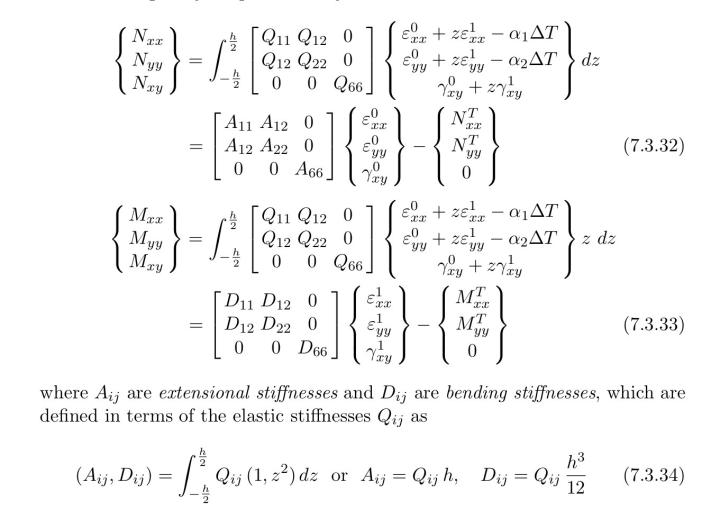
\includegraphics[width=0.55\linewidth]{Figure/fig37}  	
			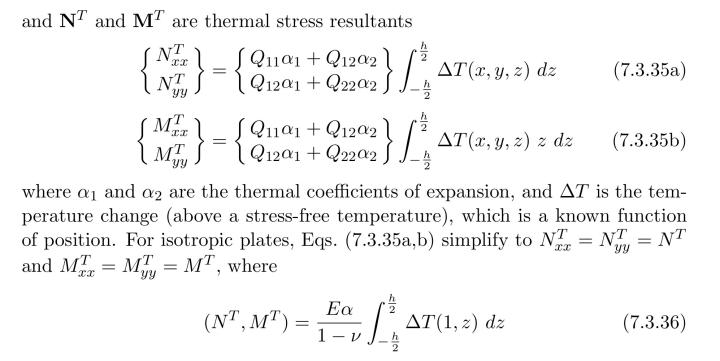
\includegraphics[width=0.4\linewidth]{Figure/fig38}	
		\end{figure}
	\end{frame}


	\begin{frame}{FEM}
		\begin{figure}
			\centering
			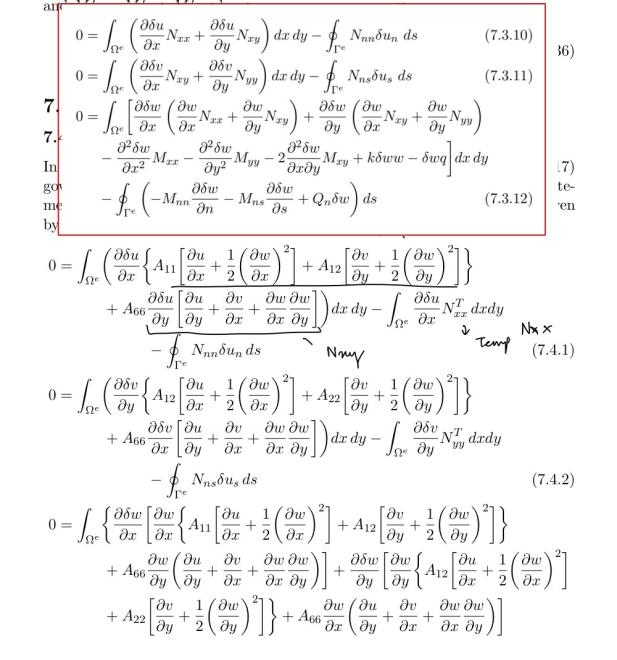
\includegraphics[width=0.6\linewidth]{Figure/fig39}  		
		\end{figure}
	\end{frame}


	\begin{frame}
		\begin{itemize}
			\item We know that $u_n,~u_s,~w,~\frac{\partial w}{\partial n}$ are used as primary variables ( or gerneralised displacements)
			\item $\hat{N_{nn}},\hat{N_{ns}},\hat{V_{n}},\hat{M_{nn}}$ as secondary degrees of greedom (generalised forces)
			\item The finite elements based on the transverse deflection $w$ and its derivative acroos element boundary (C1 conitunity). In completeness, it should be a full quadratic.
			\item $u_n$ and $u_s$ need only be C0. We shall use $u,v,w,\frac{\partial w}{\partial x}, \frac{\partial w}{\partial y}$ as the generalised displacements. We assume as
			\begin{equation}
			u(x,y) =N_i^1u_i \qquad v(x,y)=N_i^1u_i \qquad w(x,y) = N_i^2u_i
			\end{equation}
			\item In case of a rectangular element wecan take two sets of dof at each node : $u,,v,w,w_{,x},w_{,y}$ and $u,,v,w,w_{,x},w_{,y}, w_{,xy}$ called non conforming and conforming element. 
			\item  In substituting we get
			\begin{equation}
				\ve{\mat{K_{11},K_{11},K_{11};K_{21},K_{22},K_{23};K_{31},K_{32},K_{33}} \mat{u;v;\Delta} = \mat{F_1;F_2;F_3} + \mat{F_{1T};F_{ 2T};F_{3T}} }
			\end{equation}
			
		\end{itemize}
	\end{frame}


	\begin{frame}
		\begin{figure}
			\centering
			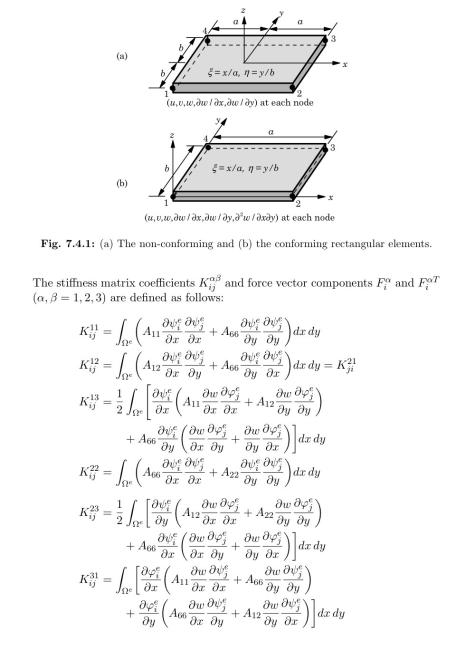
\includegraphics[width=0.4\linewidth]{Figure/fig40}  		
			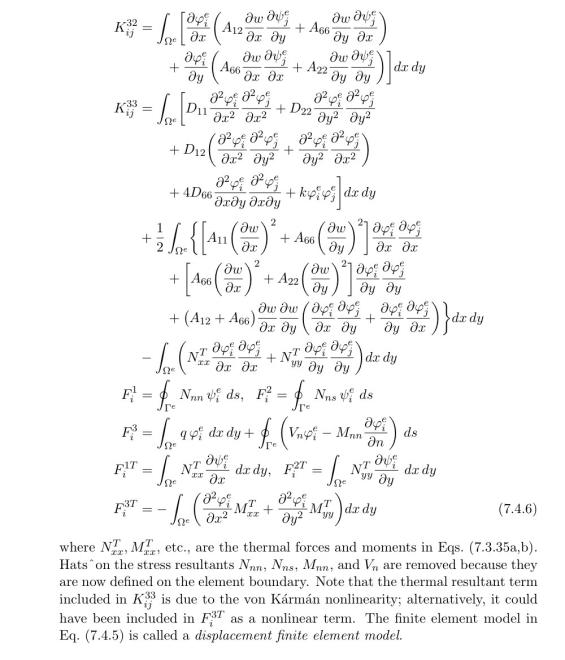
\includegraphics[width=0.4\linewidth]{Figure/fig41}
		\end{figure}
	\end{frame}


	\begin{frame}{Tangent stiffness coefficients}
		\begin{itemize}
			\item Check Tangent in Reddy 328
		\end{itemize}
	\end{frame}


	\begin{frame}{Conforming and non conforming plate elements}
		\begin{itemize}
			\item A non conforming element also has nodal variable of $w_{,x},w_{,y}$
			\item Using the parametric form we see that 
			\begin{equation}
				\begin{aligned}
				u = u_h =  u_i N^1_i(\xi,\eta) \qquad v = v_h =  v_iN^1_i(\xi,\eta) \\
				w_h = \Delta N^2_i(\xi,\eta) ~~\text{Cubic to associate with dof}~ w,w_{,x},w_{,y}\\			
				\end{aligned}
			\end{equation}
			\item The variation of the normal slope $w_{,n}$ is cubic while there are only two values of it available on the edge ()??????????.
			\item Therefore, cubic polynomials for the normal derivatives of $w$ are not the same on an edge common to two elements, hence non-conforming. I guess corner one is not the same 
			\item Conforming elemen has $w$ approximated by 16 term complete polyunomial with dof $w, w_{,x},w_{,y},w_{,xy}$
			\item Here the normal slope continuity between elements is satisfied.
			\end{itemize}
	\end{frame}


	\begin{frame}{Derivatives}
		\begin{itemize}
			\item Here we use bilinear interpolation of $u,v$ and hermite of $w$
			\item The geomettry is also represented using bilinear interpolating functions
			\begin{equation}
				x = N_i(\xi,\eta)x_i \qquad y = N_i(\xi,\eta) y_i
			\end{equation}
			\item The derivatives of the inerpolating funcction with respect to global is given by
			\begin{equation}
				\mat{\frac{\partial N_i}{\partial x}; \frac{\partial N_i}{\partial y} = J^{-1} 
					\mat{\frac{\partial N_i}{\partial \xi}; \frac{\partial N_i}{\partial \eta}}}
			\end{equation}
			\item For the second order derivatives, we can use again chain rule
			\begin{equation}
			\begin{aligned}
				\frac{\partial N_i}{\partial \xi} = \frac{\partial N_i}{\partial x}\frac{\partial  x}{\partial \xi} + \frac{\partial N_i}{\partial y}\frac{\partial  y}{\partial \xi}
				\qquad
				\frac{\partial N_i}{\partial \eta} = \frac{\partial N_i}{\partial x}\frac{\partial  x}{\partial \eta} + \frac{\partial N_i}{\partial y}\frac{\partial  y}{\partial \eta} \\
				\frac{\partial^2 N_i}{\partial \xi^2} = \frac{\partial }{\partial \xi}\left(\frac{\partial N_i}{\partial x}\frac{\partial  x}{\partial \xi} + \frac{\partial N_i}{\partial y}\frac{\partial  y}{\partial \xi} \right)		\qquad
				\frac{\partial^2 N_i}{\partial \eta^2} = \frac{\partial }{\partial \eta}\left(\frac{\partial N_i}{\partial x}\frac{\partial  x}{\partial \eta} + \frac{\partial N_i}{\partial y}\frac{\partial  y}{\partial \eta} \right)		  
			\end{aligned}
			\end{equation}
		\end{itemize}
	\end{frame}


	\begin{frame}{Stresses}
		\begin{itemize}
			\item The stresses $\sigma_{xx},\sigma_{yy},\sigma_{xy}$ are computed using stress-strain relations and computed in global coordinates using 		
		\end{itemize}
		\begin{figure}
			\centering
			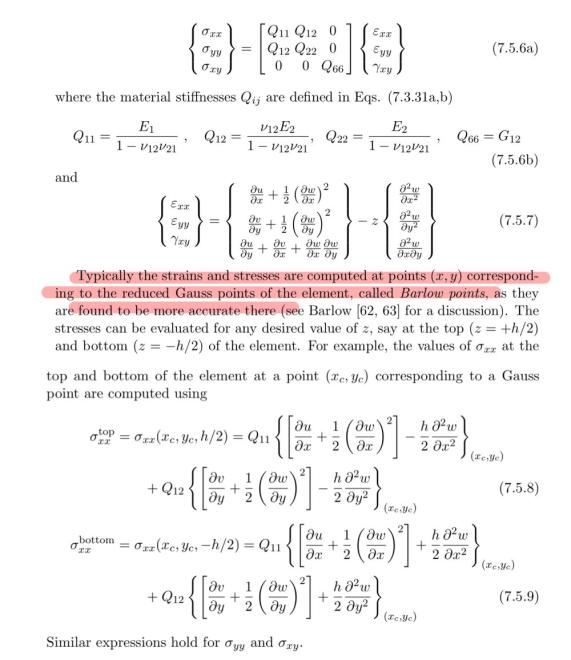
\includegraphics[width=0.5\linewidth]{Figure/fig42}  		
		\end{figure}
	\end{frame}

	
	\begin{frame}{First order shear deformation}
		\begin{itemize}
			\item Transverese normal and shear are not neglected. This formulation requires only C0 interpolation of all gerneralized displacements!
			\item Displacement field : Same assumptions of classical theroy but relaxing the normality condition
			\begin{equation}
			\begin{aligned}
				u_1(x,y,z) = u(x,y) + z\phi_x(x,y)\\
				u_2(x,y,z) = v(x,y) + z\phi_y(x,y)\\
				u_3(x,y,z) = w(x,y) 
			\end{aligned}
			\end{equation}
			\begin{figure}
				\centering
				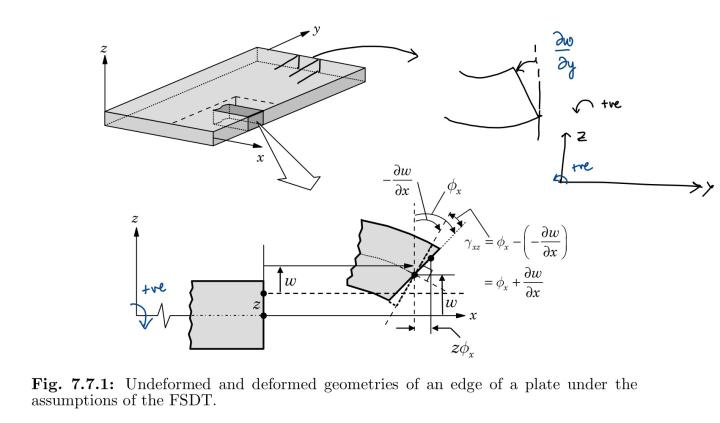
\includegraphics[width=0.55\linewidth]{Figure/fig44}  		
			\end{figure}
			\item Where ($u,v,w,\phi_x,\phi_y$) are unkown functions. $\phi_x,\phi_y$ denote the rotations of transverser normal line about y and x axes. These are called generalized displacements
		\end{itemize}
	\end{frame}


	\begin{frame}{Displacement: Continued}
		\begin{itemize}
			\item Notation that $\phi_x,\phi_y$ denoe rotation about a transverse normal about y
			\item We then get
			\begin{equation}
			\begin{aligned}
				\beta_x = -\phi_y \qquad \beta_y = \phi_x\\
				\phi_x = - \frac{\partial w}{\partial x} \qquad 				
				\phi_y = - \frac{\partial w}{\partial y} \quad \text{For thin plates of thickness ratio of order \~ O(50)}
			\end{aligned}
			\end{equation}
			\item However this equality is not achieved in the discrete fem model, resulting in shear locking as in Timoshenko beam, when the same lower order approx are used for transverse deflection $w$ and rotation $\phi$
			
		\end{itemize}
	\end{frame}


	\begin{frame}{von Karman strains}
		\begin{itemize}
			\item The von karman strains are:
			\begin{equation}
			\mat{\varepsilon_{xx};\varepsilon_{yy};\varepsilon_{yz};\varepsilon_{xz};\varepsilon_{xy}} =
			\mat{\varepsilon^0_{xx};\varepsilon^0_{yy};\varepsilon^0_{yz};\varepsilon^0_{xz};\varepsilon^0_{xy}} +
		z   \mat{\varepsilon^1_{xx};\varepsilon^1_{yy};0;0;\varepsilon^1_{xy}} =
			\mat{\frac{\partial u}{\partial x} + \frac{1}{2}(\frac{\partial w}{\partial x})^2 ; ; 
				 \frac{\partial v}{\partial y} + \frac{1}{2}(\frac{\partial w}{\partial y})^2 ; ;
			     \frac{\partial w}{\partial y} + \phi_y                                       ; ;
		     	 \frac{\partial w}{\partial x} + \phi_x                                       ; ;
	     	     \frac{\partial u}{\partial y} + \frac{\partial v}{\partial x} + \frac{\partial w}{\partial x} \frac{\partial w}{\partial y}} +
        z   \mat{\frac{\partial \phi_x}{\partial x}; ; \frac{\partial \phi_y}{\partial y}; ; 0 ; ; 0 ; ; \frac{\partial \phi_x}{\partial y} + \frac{\partial \phi_y}{\partial x}}
			\end{equation}
			\item Note that the strains ($\varepsilon_{xx,yy,xy}$) are linear through the plate thickness while the transverse strains ($\gamma_{xz},\gamma_{yz}$) are constant.
		\end{itemize}
	\end{frame}


	\begin{frame}{Weak form using virtual work}
		\begin{itemize}
			\item The weak form for $\delta W_I$ and $\delta W_E$ is :
			\begin{figure}
				\centering
				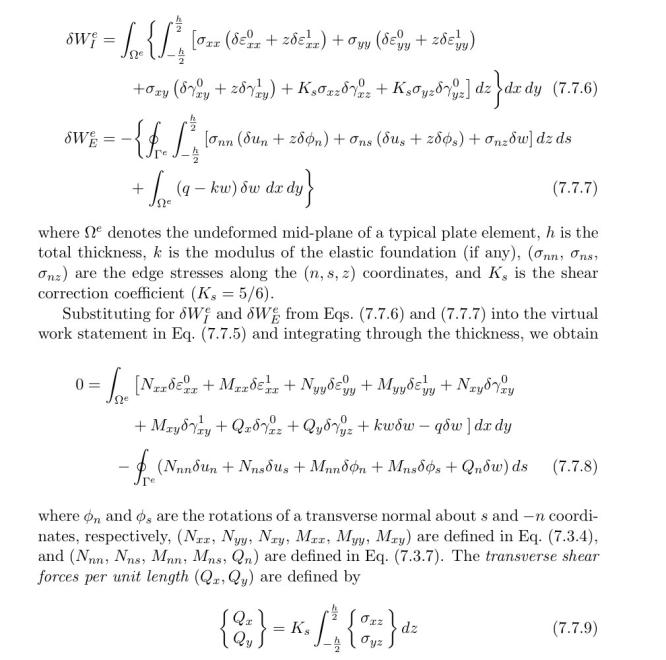
\includegraphics[width=0.7\linewidth]{Figure/fig45}  		
			\end{figure}
		\end{itemize}
	\end{frame}


	\begin{frame}{Governing equationbs}
		\begin{itemize}
			\item The virtual work equation contains five different statements associated with five virtual displacements ($\delta u, \delta v, \delta w, \delta \phi_x, \delta \phi_y$) forming the basis of the fem model
			\item The governing equations not required for fem, are shown as done previously by removing all the virtual displacments of differentiation. We then get:
		\end{itemize}
	\end{frame}


	\begin{frame}
		\begin{figure}
			\centering
			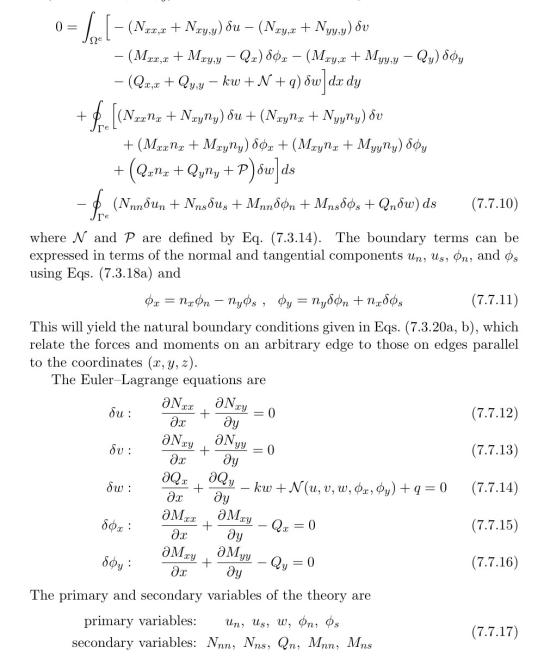
\includegraphics[width=0.65\linewidth]{Figure/fig46}  		
		\end{figure}
	\end{frame}


	\begin{frame}
		\begin{itemize}
			\item Since the transverse shear strains are constant, the shear stresses will also be constant. But the transverse shear stress is actually parabolic, whihc is taken care using a shape factor on the shear stiffness. 
			\begin{figure}
				\centering
				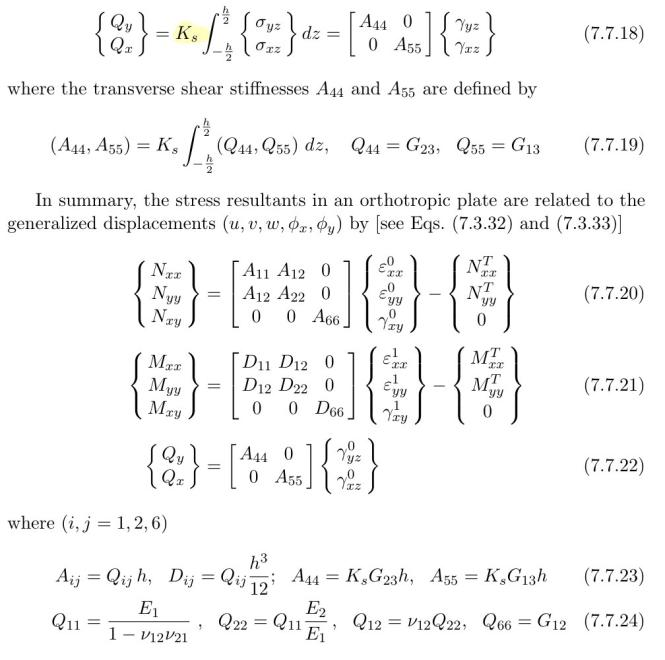
\includegraphics[width=0.65\linewidth]{Figure/fig47}  		
			\end{figure}
			\item As you can see that once you have the shear deformation, we change how G (shear modulus is)
		\end{itemize}
	\end{frame}


	\begin{frame}{FEM models of FSDT}
		\begin{itemize}
			\item FEM model
			\item  The rotationsa ($\phi$) are independant of $w$. So no derivatives appear and all the  generalized displafcements can be interpolated using Largrange interpolating functions.
			\item Tangent matrix : See Reddy
			
		\end{itemize}
	\end{frame}


	\begin{frame}{Shear and membrane locking and transient}
		\begin{itemize}
			\item The lienarised interpolation of the generalized displcamnets is used, making the element very stiff in the thin plate limit. This is called shear locking. A common technique is to use selective integration. Reduced integration is used to evalueate all the transeverse shear stiffnesses.			
			\item \textbf{Transient:}Check Reddy
	\end{itemize}
	\end{frame}


\section{Nonlinear bending of shells}

	
	\begin{frame}{Introduction}
		\begin{itemize}
			\item Shells are much like plates except that they are curved. 
			\item FEM models of shells are developed using (1) shell theory or (2) 2-D equations obtained from a degenerated 3D elasticity model 
			\item Shell theory are developed, are origninally based on Kirchoff-Love kinematic hypothesis
			\item Some group of shell theories is based on order magnitude on strains and rotations in full nonlinear equations (called finite rotation theories). 
			\begin{itemize}
				\item Strains and rotations about the normal to he surface are assumed to be of order $\epsilon<<1$
				\item Roations about tangents to the surface are organised in a consistent classiciation where for each range of magnitude of ratioans specific shell euqations are obtained. 
			\end{itemize}
		\item Shells can be synclastic or anticlastic. A curved surface is developable if it can be developed to a plane without sretching. Nondevelopable requires cuting or deforming. These are stronger than developable because they need additional forces to collapse to planar surfaces. 
		\end{itemize}
	\end{frame}


	\begin{frame}{Governing equations}
		\begin{figure}
			\centering
			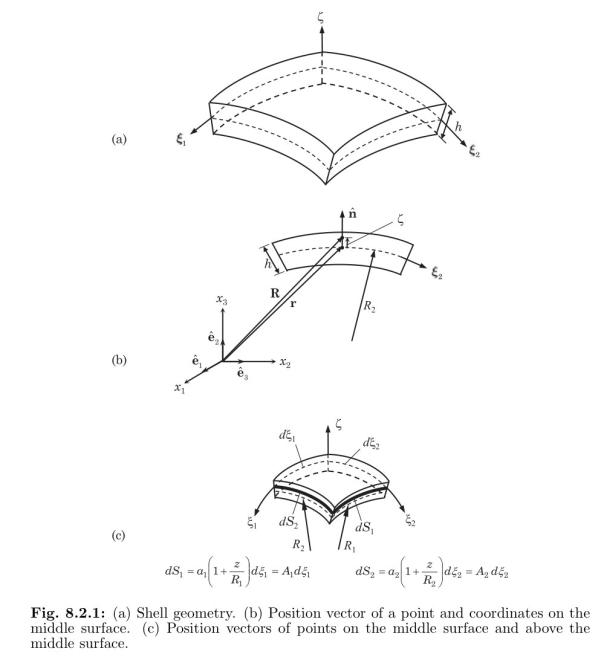
\includegraphics[width=0.65\linewidth]{Figure/fig48}  		
		\end{figure}
	\end{frame}


	\begin{frame}{Differential geometry}
		\begin{itemize}
			\item Take a curved shell element of uniform thickness. Here ($\xi_1,\xi_2,\zeta$) which denote the curvilinear coordinates such that $\xi_1, \xi_2$ curves are the lines of crvature of the middle surface ($\zeta = 0$). 
			\item The position vector of a point ($\xi_1,\xi_2,0$) is denote by $\ve{r}$ and any other arbitary point is denoted by $\ve{R}$
			\item A differential line element on the middle suface can be written as 
			\begin{equation}
			d\ve{r} = \frac{\partial \ve{r}}{\partial \xi_a}d\xi_a = \ve{g}_a d\xi_a , \quad \ve{g}_a = \frac{\partial \ve{r}}{\partial \xi_a} \quad (a =1,2)
			\end{equation}
			where the vectors $\ve{g}_1$ and $\ve{g}_2$ are tangent to the $\xi_1,\xi_2$ coordinates lines as shown.
			\item  The components of the metric tensor $g_{ab}$, (a,b=1,2) are 
			\begin{equation}
			\ve{g}_a.\ve{g}_b = g_{ab},  \qquad p_1 = \sqrt{g_{11}}, \qquad p_2 = \sqrt{g_{22}}, \qquad \ve{g_1.g_2} = p_1p_2cos \chi
			\end{equation}
			where $\chi$ denotes the angle between the coordinate curves. \footnote{Note that $\ve{\hat{n}},p_1,p_2$ are functions of $\xi_1,\xi_2$}
			\item The normal vector is found as
			\begin{equation}
			\ve{\hat{n}} = \frac{\ve{g_1 \times g_2}}{p_1p_2sin \chi}
			\end{equation}
		\end{itemize}	
	\end{frame}


	\begin{frame}{Differential geometry : continued}
		\begin{itemize}
			\item The square of the distance $dS$,say between points ($\xi_1,\xi_2,0$) and ($\xi_1 + d\xi_1,\xi_2+d\xi_2,0$) on th emiddle surface is given by
			\begin{equation}
			 (ds)^2 = d\ve{r}. d\ve{r} = g_{ab}d\xi_a d\xi_b = p_1^2(d\xi_1)^2 + p_2^2(d\xi_2)^2 + 2a_1a_2cos~\chi~d\xi_1 d\xi_2
			\end{equation}
			The RHS is called the first quadratic form of the surface which allows us to find infinitesimal lengths, angles and area. The terms $p_1^2,~p_2^2,~p_1p_2cos\chi$ are called the first fundamental quantities
			\item Let $\ve{r}= \ve{r}(s)$ be the equation of a curve $s$ on the surface. The unit vector tangent to the curve is
			\begin{equation}
				\ve{\hat{t}} =  \frac{d \ve{r}}{d   s} = \frac{\partial \ve{r}}{\partial \xi_a} \frac{\partial \xi_a}{\partial s} = \ve{g}_a \frac{\partial \xi_a}{\partial s}
			\end{equation}			
		\end{itemize}
	\end{frame}


	\begin{frame}{Governing E}
		Im not writing this because the conventions are too long. Please check the annotated book
	\end{frame}